\documentclass{article} % For LaTeX2e
\usepackage{iclr2022_conference,times}

% Optional math commands from https://github.com/goodfeli/dlbook_notation.
%%%%% NEW MATH DEFINITIONS %%%%%

\usepackage{amsmath,amsfonts,bm}

% Mark sections of captions for referring to divisions of figures
\newcommand{\figleft}{{\em (Left)}}
\newcommand{\figcenter}{{\em (Center)}}
\newcommand{\figright}{{\em (Right)}}
\newcommand{\figtop}{{\em (Top)}}
\newcommand{\figbottom}{{\em (Bottom)}}
\newcommand{\captiona}{{\em (a)}}
\newcommand{\captionb}{{\em (b)}}
\newcommand{\captionc}{{\em (c)}}
\newcommand{\captiond}{{\em (d)}}

% Highlight a newly defined term
\newcommand{\newterm}[1]{{\bf #1}}


% Figure reference, lower-case.
\def\figref#1{figure~\ref{#1}}
% Figure reference, capital. For start of sentence
\def\Figref#1{Figure~\ref{#1}}
\def\twofigref#1#2{figures \ref{#1} and \ref{#2}}
\def\quadfigref#1#2#3#4{figures \ref{#1}, \ref{#2}, \ref{#3} and \ref{#4}}
% Section reference, lower-case.
\def\secref#1{section~\ref{#1}}
% Section reference, capital.
\def\Secref#1{Section~\ref{#1}}
% Reference to two sections.
\def\twosecrefs#1#2{sections \ref{#1} and \ref{#2}}
% Reference to three sections.
\def\secrefs#1#2#3{sections \ref{#1}, \ref{#2} and \ref{#3}}
% Reference to an equation, lower-case.
\def\eqref#1{equation~\ref{#1}}
% Reference to an equation, upper case
\def\Eqref#1{Equation~\ref{#1}}
% A raw reference to an equation---avoid using if possible
\def\plaineqref#1{\ref{#1}}
% Reference to a chapter, lower-case.
\def\chapref#1{chapter~\ref{#1}}
% Reference to an equation, upper case.
\def\Chapref#1{Chapter~\ref{#1}}
% Reference to a range of chapters
\def\rangechapref#1#2{chapters\ref{#1}--\ref{#2}}
% Reference to an algorithm, lower-case.
\def\algref#1{algorithm~\ref{#1}}
% Reference to an algorithm, upper case.
\def\Algref#1{Algorithm~\ref{#1}}
\def\twoalgref#1#2{algorithms \ref{#1} and \ref{#2}}
\def\Twoalgref#1#2{Algorithms \ref{#1} and \ref{#2}}
% Reference to a part, lower case
\def\partref#1{part~\ref{#1}}
% Reference to a part, upper case
\def\Partref#1{Part~\ref{#1}}
\def\twopartref#1#2{parts \ref{#1} and \ref{#2}}

\def\ceil#1{\lceil #1 \rceil}
\def\floor#1{\lfloor #1 \rfloor}
\def\1{\bm{1}}
\newcommand{\train}{\mathcal{D}}
\newcommand{\valid}{\mathcal{D_{\mathrm{valid}}}}
\newcommand{\test}{\mathcal{D_{\mathrm{test}}}}

\def\eps{{\epsilon}}


% Random variables
\def\reta{{\textnormal{$\eta$}}}
\def\ra{{\textnormal{a}}}
\def\rb{{\textnormal{b}}}
\def\rc{{\textnormal{c}}}
\def\rd{{\textnormal{d}}}
\def\re{{\textnormal{e}}}
\def\rf{{\textnormal{f}}}
\def\rg{{\textnormal{g}}}
\def\rh{{\textnormal{h}}}
\def\ri{{\textnormal{i}}}
\def\rj{{\textnormal{j}}}
\def\rk{{\textnormal{k}}}
\def\rl{{\textnormal{l}}}
% rm is already a command, just don't name any random variables m
\def\rn{{\textnormal{n}}}
\def\ro{{\textnormal{o}}}
\def\rp{{\textnormal{p}}}
\def\rq{{\textnormal{q}}}
\def\rr{{\textnormal{r}}}
\def\rs{{\textnormal{s}}}
\def\rt{{\textnormal{t}}}
\def\ru{{\textnormal{u}}}
\def\rv{{\textnormal{v}}}
\def\rw{{\textnormal{w}}}
\def\rx{{\textnormal{x}}}
\def\ry{{\textnormal{y}}}
\def\rz{{\textnormal{z}}}

% Random vectors
\def\rvepsilon{{\mathbf{\epsilon}}}
\def\rvtheta{{\mathbf{\theta}}}
\def\rva{{\mathbf{a}}}
\def\rvb{{\mathbf{b}}}
\def\rvc{{\mathbf{c}}}
\def\rvd{{\mathbf{d}}}
\def\rve{{\mathbf{e}}}
\def\rvf{{\mathbf{f}}}
\def\rvg{{\mathbf{g}}}
\def\rvh{{\mathbf{h}}}
\def\rvu{{\mathbf{i}}}
\def\rvj{{\mathbf{j}}}
\def\rvk{{\mathbf{k}}}
\def\rvl{{\mathbf{l}}}
\def\rvm{{\mathbf{m}}}
\def\rvn{{\mathbf{n}}}
\def\rvo{{\mathbf{o}}}
\def\rvp{{\mathbf{p}}}
\def\rvq{{\mathbf{q}}}
\def\rvr{{\mathbf{r}}}
\def\rvs{{\mathbf{s}}}
\def\rvt{{\mathbf{t}}}
\def\rvu{{\mathbf{u}}}
\def\rvv{{\mathbf{v}}}
\def\rvw{{\mathbf{w}}}
\def\rvx{{\mathbf{x}}}
\def\rvy{{\mathbf{y}}}
\def\rvz{{\mathbf{z}}}

% Elements of random vectors
\def\erva{{\textnormal{a}}}
\def\ervb{{\textnormal{b}}}
\def\ervc{{\textnormal{c}}}
\def\ervd{{\textnormal{d}}}
\def\erve{{\textnormal{e}}}
\def\ervf{{\textnormal{f}}}
\def\ervg{{\textnormal{g}}}
\def\ervh{{\textnormal{h}}}
\def\ervi{{\textnormal{i}}}
\def\ervj{{\textnormal{j}}}
\def\ervk{{\textnormal{k}}}
\def\ervl{{\textnormal{l}}}
\def\ervm{{\textnormal{m}}}
\def\ervn{{\textnormal{n}}}
\def\ervo{{\textnormal{o}}}
\def\ervp{{\textnormal{p}}}
\def\ervq{{\textnormal{q}}}
\def\ervr{{\textnormal{r}}}
\def\ervs{{\textnormal{s}}}
\def\ervt{{\textnormal{t}}}
\def\ervu{{\textnormal{u}}}
\def\ervv{{\textnormal{v}}}
\def\ervw{{\textnormal{w}}}
\def\ervx{{\textnormal{x}}}
\def\ervy{{\textnormal{y}}}
\def\ervz{{\textnormal{z}}}

% Random matrices
\def\rmA{{\mathbf{A}}}
\def\rmB{{\mathbf{B}}}
\def\rmC{{\mathbf{C}}}
\def\rmD{{\mathbf{D}}}
\def\rmE{{\mathbf{E}}}
\def\rmF{{\mathbf{F}}}
\def\rmG{{\mathbf{G}}}
\def\rmH{{\mathbf{H}}}
\def\rmI{{\mathbf{I}}}
\def\rmJ{{\mathbf{J}}}
\def\rmK{{\mathbf{K}}}
\def\rmL{{\mathbf{L}}}
\def\rmM{{\mathbf{M}}}
\def\rmN{{\mathbf{N}}}
\def\rmO{{\mathbf{O}}}
\def\rmP{{\mathbf{P}}}
\def\rmQ{{\mathbf{Q}}}
\def\rmR{{\mathbf{R}}}
\def\rmS{{\mathbf{S}}}
\def\rmT{{\mathbf{T}}}
\def\rmU{{\mathbf{U}}}
\def\rmV{{\mathbf{V}}}
\def\rmW{{\mathbf{W}}}
\def\rmX{{\mathbf{X}}}
\def\rmY{{\mathbf{Y}}}
\def\rmZ{{\mathbf{Z}}}

% Elements of random matrices
\def\ermA{{\textnormal{A}}}
\def\ermB{{\textnormal{B}}}
\def\ermC{{\textnormal{C}}}
\def\ermD{{\textnormal{D}}}
\def\ermE{{\textnormal{E}}}
\def\ermF{{\textnormal{F}}}
\def\ermG{{\textnormal{G}}}
\def\ermH{{\textnormal{H}}}
\def\ermI{{\textnormal{I}}}
\def\ermJ{{\textnormal{J}}}
\def\ermK{{\textnormal{K}}}
\def\ermL{{\textnormal{L}}}
\def\ermM{{\textnormal{M}}}
\def\ermN{{\textnormal{N}}}
\def\ermO{{\textnormal{O}}}
\def\ermP{{\textnormal{P}}}
\def\ermQ{{\textnormal{Q}}}
\def\ermR{{\textnormal{R}}}
\def\ermS{{\textnormal{S}}}
\def\ermT{{\textnormal{T}}}
\def\ermU{{\textnormal{U}}}
\def\ermV{{\textnormal{V}}}
\def\ermW{{\textnormal{W}}}
\def\ermX{{\textnormal{X}}}
\def\ermY{{\textnormal{Y}}}
\def\ermZ{{\textnormal{Z}}}

% Vectors
\def\vzero{{\bm{0}}}
\def\vone{{\bm{1}}}
\def\vmu{{\bm{\mu}}}
\def\vtheta{{\bm{\theta}}}
\def\va{{\bm{a}}}
\def\vb{{\bm{b}}}
\def\vc{{\bm{c}}}
\def\vd{{\bm{d}}}
\def\ve{{\bm{e}}}
\def\vf{{\bm{f}}}
\def\vg{{\bm{g}}}
\def\vh{{\bm{h}}}
\def\vi{{\bm{i}}}
\def\vj{{\bm{j}}}
\def\vk{{\bm{k}}}
\def\vl{{\bm{l}}}
\def\vm{{\bm{m}}}
\def\vn{{\bm{n}}}
\def\vo{{\bm{o}}}
\def\vp{{\bm{p}}}
\def\vq{{\bm{q}}}
\def\vr{{\bm{r}}}
\def\vs{{\bm{s}}}
\def\vt{{\bm{t}}}
\def\vu{{\bm{u}}}
\def\vv{{\bm{v}}}
\def\vw{{\bm{w}}}
\def\vx{{\bm{x}}}
\def\vy{{\bm{y}}}
\def\vz{{\bm{z}}}

% Elements of vectors
\def\evalpha{{\alpha}}
\def\evbeta{{\beta}}
\def\evepsilon{{\epsilon}}
\def\evlambda{{\lambda}}
\def\evomega{{\omega}}
\def\evmu{{\mu}}
\def\evpsi{{\psi}}
\def\evsigma{{\sigma}}
\def\evtheta{{\theta}}
\def\eva{{a}}
\def\evb{{b}}
\def\evc{{c}}
\def\evd{{d}}
\def\eve{{e}}
\def\evf{{f}}
\def\evg{{g}}
\def\evh{{h}}
\def\evi{{i}}
\def\evj{{j}}
\def\evk{{k}}
\def\evl{{l}}
\def\evm{{m}}
\def\evn{{n}}
\def\evo{{o}}
\def\evp{{p}}
\def\evq{{q}}
\def\evr{{r}}
\def\evs{{s}}
\def\evt{{t}}
\def\evu{{u}}
\def\evv{{v}}
\def\evw{{w}}
\def\evx{{x}}
\def\evy{{y}}
\def\evz{{z}}

% Matrix
\def\mA{{\bm{A}}}
\def\mB{{\bm{B}}}
\def\mC{{\bm{C}}}
\def\mD{{\bm{D}}}
\def\mE{{\bm{E}}}
\def\mF{{\bm{F}}}
\def\mG{{\bm{G}}}
\def\mH{{\bm{H}}}
\def\mI{{\bm{I}}}
\def\mJ{{\bm{J}}}
\def\mK{{\bm{K}}}
\def\mL{{\bm{L}}}
\def\mM{{\bm{M}}}
\def\mN{{\bm{N}}}
\def\mO{{\bm{O}}}
\def\mP{{\bm{P}}}
\def\mQ{{\bm{Q}}}
\def\mR{{\bm{R}}}
\def\mS{{\bm{S}}}
\def\mT{{\bm{T}}}
\def\mU{{\bm{U}}}
\def\mV{{\bm{V}}}
\def\mW{{\bm{W}}}
\def\mX{{\bm{X}}}
\def\mY{{\bm{Y}}}
\def\mZ{{\bm{Z}}}
\def\mBeta{{\bm{\beta}}}
\def\mPhi{{\bm{\Phi}}}
\def\mLambda{{\bm{\Lambda}}}
\def\mSigma{{\bm{\Sigma}}}

% Tensor
\DeclareMathAlphabet{\mathsfit}{\encodingdefault}{\sfdefault}{m}{sl}
\SetMathAlphabet{\mathsfit}{bold}{\encodingdefault}{\sfdefault}{bx}{n}
\newcommand{\tens}[1]{\bm{\mathsfit{#1}}}
\def\tA{{\tens{A}}}
\def\tB{{\tens{B}}}
\def\tC{{\tens{C}}}
\def\tD{{\tens{D}}}
\def\tE{{\tens{E}}}
\def\tF{{\tens{F}}}
\def\tG{{\tens{G}}}
\def\tH{{\tens{H}}}
\def\tI{{\tens{I}}}
\def\tJ{{\tens{J}}}
\def\tK{{\tens{K}}}
\def\tL{{\tens{L}}}
\def\tM{{\tens{M}}}
\def\tN{{\tens{N}}}
\def\tO{{\tens{O}}}
\def\tP{{\tens{P}}}
\def\tQ{{\tens{Q}}}
\def\tR{{\tens{R}}}
\def\tS{{\tens{S}}}
\def\tT{{\tens{T}}}
\def\tU{{\tens{U}}}
\def\tV{{\tens{V}}}
\def\tW{{\tens{W}}}
\def\tX{{\tens{X}}}
\def\tY{{\tens{Y}}}
\def\tZ{{\tens{Z}}}


% Graph
\def\gA{{\mathcal{A}}}
\def\gB{{\mathcal{B}}}
\def\gC{{\mathcal{C}}}
\def\gD{{\mathcal{D}}}
\def\gE{{\mathcal{E}}}
\def\gF{{\mathcal{F}}}
\def\gG{{\mathcal{G}}}
\def\gH{{\mathcal{H}}}
\def\gI{{\mathcal{I}}}
\def\gJ{{\mathcal{J}}}
\def\gK{{\mathcal{K}}}
\def\gL{{\mathcal{L}}}
\def\gM{{\mathcal{M}}}
\def\gN{{\mathcal{N}}}
\def\gO{{\mathcal{O}}}
\def\gP{{\mathcal{P}}}
\def\gQ{{\mathcal{Q}}}
\def\gR{{\mathcal{R}}}
\def\gS{{\mathcal{S}}}
\def\gT{{\mathcal{T}}}
\def\gU{{\mathcal{U}}}
\def\gV{{\mathcal{V}}}
\def\gW{{\mathcal{W}}}
\def\gX{{\mathcal{X}}}
\def\gY{{\mathcal{Y}}}
\def\gZ{{\mathcal{Z}}}

% Sets
\def\sA{{\mathbb{A}}}
\def\sB{{\mathbb{B}}}
\def\sC{{\mathbb{C}}}
\def\sD{{\mathbb{D}}}
% Don't use a set called E, because this would be the same as our symbol
% for expectation.
\def\sF{{\mathbb{F}}}
\def\sG{{\mathbb{G}}}
\def\sH{{\mathbb{H}}}
\def\sI{{\mathbb{I}}}
\def\sJ{{\mathbb{J}}}
\def\sK{{\mathbb{K}}}
\def\sL{{\mathbb{L}}}
\def\sM{{\mathbb{M}}}
\def\sN{{\mathbb{N}}}
\def\sO{{\mathbb{O}}}
\def\sP{{\mathbb{P}}}
\def\sQ{{\mathbb{Q}}}
\def\sR{{\mathbb{R}}}
\def\sS{{\mathbb{S}}}
\def\sT{{\mathbb{T}}}
\def\sU{{\mathbb{U}}}
\def\sV{{\mathbb{V}}}
\def\sW{{\mathbb{W}}}
\def\sX{{\mathbb{X}}}
\def\sY{{\mathbb{Y}}}
\def\sZ{{\mathbb{Z}}}

% Entries of a matrix
\def\emLambda{{\Lambda}}
\def\emA{{A}}
\def\emB{{B}}
\def\emC{{C}}
\def\emD{{D}}
\def\emE{{E}}
\def\emF{{F}}
\def\emG{{G}}
\def\emH{{H}}
\def\emI{{I}}
\def\emJ{{J}}
\def\emK{{K}}
\def\emL{{L}}
\def\emM{{M}}
\def\emN{{N}}
\def\emO{{O}}
\def\emP{{P}}
\def\emQ{{Q}}
\def\emR{{R}}
\def\emS{{S}}
\def\emT{{T}}
\def\emU{{U}}
\def\emV{{V}}
\def\emW{{W}}
\def\emX{{X}}
\def\emY{{Y}}
\def\emZ{{Z}}
\def\emSigma{{\Sigma}}

% entries of a tensor
% Same font as tensor, without \bm wrapper
\newcommand{\etens}[1]{\mathsfit{#1}}
\def\etLambda{{\etens{\Lambda}}}
\def\etA{{\etens{A}}}
\def\etB{{\etens{B}}}
\def\etC{{\etens{C}}}
\def\etD{{\etens{D}}}
\def\etE{{\etens{E}}}
\def\etF{{\etens{F}}}
\def\etG{{\etens{G}}}
\def\etH{{\etens{H}}}
\def\etI{{\etens{I}}}
\def\etJ{{\etens{J}}}
\def\etK{{\etens{K}}}
\def\etL{{\etens{L}}}
\def\etM{{\etens{M}}}
\def\etN{{\etens{N}}}
\def\etO{{\etens{O}}}
\def\etP{{\etens{P}}}
\def\etQ{{\etens{Q}}}
\def\etR{{\etens{R}}}
\def\etS{{\etens{S}}}
\def\etT{{\etens{T}}}
\def\etU{{\etens{U}}}
\def\etV{{\etens{V}}}
\def\etW{{\etens{W}}}
\def\etX{{\etens{X}}}
\def\etY{{\etens{Y}}}
\def\etZ{{\etens{Z}}}

% The true underlying data generating distribution
\newcommand{\pdata}{p_{\rm{data}}}
% The empirical distribution defined by the training set
\newcommand{\ptrain}{\hat{p}_{\rm{data}}}
\newcommand{\Ptrain}{\hat{P}_{\rm{data}}}
% The model distribution
\newcommand{\pmodel}{p_{\rm{model}}}
\newcommand{\Pmodel}{P_{\rm{model}}}
\newcommand{\ptildemodel}{\tilde{p}_{\rm{model}}}
% Stochastic autoencoder distributions
\newcommand{\pencode}{p_{\rm{encoder}}}
\newcommand{\pdecode}{p_{\rm{decoder}}}
\newcommand{\precons}{p_{\rm{reconstruct}}}

\newcommand{\laplace}{\mathrm{Laplace}} % Laplace distribution

\newcommand{\E}{\mathbb{E}}
\newcommand{\Ls}{\mathcal{L}}
\newcommand{\R}{\mathbb{R}}
\newcommand{\emp}{\tilde{p}}
\newcommand{\lr}{\alpha}
\newcommand{\reg}{\lambda}
\newcommand{\rect}{\mathrm{rectifier}}
\newcommand{\softmax}{\mathrm{softmax}}
\newcommand{\sigmoid}{\sigma}
\newcommand{\softplus}{\zeta}
\newcommand{\KL}{D_{\mathrm{KL}}}
\newcommand{\Var}{\mathrm{Var}}
\newcommand{\standarderror}{\mathrm{SE}}
\newcommand{\Cov}{\mathrm{Cov}}
% Wolfram Mathworld says $L^2$ is for function spaces and $\ell^2$ is for vectors
% But then they seem to use $L^2$ for vectors throughout the site, and so does
% wikipedia.
\newcommand{\normlzero}{L^0}
\newcommand{\normlone}{L^1}
\newcommand{\normltwo}{L^2}
\newcommand{\normlp}{L^p}
\newcommand{\normmax}{L^\infty}

\newcommand{\parents}{Pa} % See usage in notation.tex. Chosen to match Daphne's book.

\DeclareMathOperator*{\argmax}{arg\,max}
\DeclareMathOperator*{\argmin}{arg\,min}

\DeclareMathOperator{\sign}{sign}
\DeclareMathOperator{\Tr}{Tr}
\let\ab\allowbreak


\usepackage[colorlinks,linkcolor=red,filecolor=blue,citecolor=blue,urlcolor=blue]{hyperref}
\usepackage{url}
\usepackage{booktabs}       % professional-quality tables
\usepackage{amsfonts}       % blackboard math symbols
\usepackage{amsmath}
\usepackage{graphicx}
\usepackage{amsthm}
\usepackage{amssymb}
\usepackage{multirow}
\usepackage{makecell}
\usepackage{algpseudocode}
\usepackage{algorithm}
% \usepackage[round]{natbib}
\usepackage{amssymb}% 
\usepackage{mathtools}
\usepackage{stmaryrd}
\usepackage[T1]{fontenc}
\usepackage{xargs}
\usepackage{xcolor}
\usepackage{wrapfig}


\def\M{\mathcal{M}}
\def\A{\mathcal{A}}
\def\Z{\mathcal{Z}}
\def\S{\mathcal{S}}
\def\D{\mathcal{D}}
\def\R{\mathcal{R}}
\def\P{\mathcal{P}}
\def\K{\mathcal{K}}
\def\E{\mathbb{E}}
\def\F{\mathfrak{F}}
\def\l{\boldsymbol{\ell}}
\newtheorem{Fact}{Fact}
\newtheorem{Lemma}{Lemma}
\newtheorem{Prop}{Proposition}
\newtheorem{definition}{Definition}
\newtheorem{Theorem}{Theorem} 
\newtheorem{Def}{Definition}
\newtheorem{Corollary}{Corollary}
\newtheorem{Conjecture}{Conjecture}
\newtheorem{Property}{Property}
\newtheorem{Observation}{Observation}
\newtheorem{Exa}{Example}
\newtheorem{assumption}{Assumption}
\newtheorem{Remark}{Remark}
\newtheorem*{Lemma*}{Lemma}
\newtheorem*{Theorem*}{Theorem}
\newtheorem*{Corollary*}{Corollary}
\newcommand{\eqsp}{\;}
\newcommand{\beq}{\begin{equation}}
\newcommand{\eeq}{\end{equation}}
\newcommand{\eqdef}{\mathrel{\mathop:}=}
\def\EE{\mathbb{E}}
\newcommand{\norm}[1]{\left\Vert #1 \right\Vert}
\newcommand{\pscal}[2]{\left\langle#1\,|\,#2 \right\rangle}
\def\major{\mathsf{M}}
\def\rset{\ensuremath{\mathbb{R}}}
\newcommand{\inter}{\llbracket n \rrbracket}
\newcommand{\interl}{\llbracket L \rrbracket}
\def\tot{\mathsf{L}}
\def\maxiter{T}
\newcommand{\ie}{{\em i.e.,~}}
\newcommand{\eg}{{\em e.g.,~}}
\newcommand{\algo}{\textsc{Comp-AMS}}



\title{On Distributed Adaptive Optimization with Gradient Compression}

% Authors must not appear in the submitted version. They should be hidden
% as long as the \iclrfinalcopy macro remains commented out below.
% Non-anonymous submissions will be rejected without review.

% \author{Antiquus S.~Hippocampus, Natalia Cerebro \& Amelie P. Amygdale \thanks{ Use footnote for providing further information
% about author (webpage, alternative address)---\emph{not} for acknowledging
% funding agencies.  Funding acknowledgements go at the end of the paper.} \\
% Department of Computer Science\\
% Cranberry-Lemon University\\
% Pittsburgh, PA 15213, USA \\
% \texttt{\{hippo,brain,jen\}@cs.cranberry-lemon.edu} \\
% \And
% Ji Q. Ren \& Yevgeny LeNet \\
% Department of Computational Neuroscience \\
% University of the Witwatersrand \\
% Joburg, South Africa \\
% \texttt{\{robot,net\}@wits.ac.za} \\
% \AND
% Coauthor \\
% Affiliation \\
% Address \\
% \texttt{email}
% }

\author{Anonymous Authors}

% The \author macro works with any number of authors. There are two commands
% used to separate the names and addresses of multiple authors: \And and \AND.
%
% Using \And between authors leaves it to \LaTeX{} to determine where to break
% the lines. Using \AND forces a linebreak at that point. So, if \LaTeX{}
% puts 3 of 4 authors names on the first line, and the last on the second
% line, try using \AND instead of \And before the third author name.

\newcommand{\fix}{\marginpar{FIX}}
\newcommand{\new}{\marginpar{NEW}}

%\iclrfinalcopy % Uncomment for camera-ready version, but NOT for submission.
\begin{document}


\maketitle


\begin{abstract}
We study \algo, a distributed optimization framework based on gradient averaging and adaptive AMSGrad algorithm. Gradient compression is applied to reduce the communication in the gradient transmission process, whose bias is corrected by the tool of error feedback. Our convergence analysis of \algo\ shows that such gradient averaging strategy yields same convergence rate as standard AMSGrad, and also exhibits linear speedup effect w.r.t. the number of local workers. Compared with recently proposed protocols on distributed adaptive methods, \algo is simple and convenient. Numerical experiments are conducted to justify the theoretical findings, and demonstrate that the proposed method can achieve same test accuracy as full-gradient AMSGrad with substantial communication savings. With its simplicity and efficiency, \algo can serve as a useful distributed training framework for adaptive methods.
\end{abstract}



\section{Introduction}\label{sec:introduction}


Deep neural network has achieved the state-of-the-art learning performance on numerous AI applications, e.g., computer vision~\citep{Proc:GAN_NIPS14,Proc:Resnet_CVPR16,CV_review18}, Natural Language Processing~\citep{Proc:Graves_ICASSP13,NLP_review18,sentiment_review18}, Reinforcement Learning~\citep{Arxiv:MnihKSGAWR13,AlphaGo_17} and recommendation systems~\citep{Proc:Covington_2016,Article:Wei_2017}. 
With the increasing sheet size of data observations and growing complexity of deep neural networks, standard single-machine training procedures encounter at least two major challenges:
\begin{itemize}
    \item Due to the limited computing power of a single-machine, processing the massive number of data samples takes a long time --- training is too slow. Many real-world applications can not even afford spending that much time on training.
  
    \item In many scenarios, data are stored in multiple servers, possibly at different locations, due to the storage constraints (massive user behavior data, Internet images, etc.) or privacy reasons~\citep{Proc:Chang18}. 
    Hence, transmitting data among servers might be costly.
\end{itemize}
\textit{Distributed learning} framework~\citep{Proc:Dean_NIPS12} has been a common training strategy to tackle the above two issues. For example, in centralized distributed stochastic gradient descent (SGD) protocol, data are located at $n$ local nodes, at which the gradients of the model are computed in parallel. In each iteration, a central server aggregates the local gradients, updates the global model, and transmits back the updated model to the local nodes for subsequent gradient computation. As we can see, this setting naturally solves aforementioned issues: 1) We use $n$ computing nodes to train the model, so the time per training epoch can be largely reduced; 2) There is no need to transmit the local data to central server. Besides, distributed training also provides stronger error tolerance since the training process could continue even one local machine breaks down. As a result of these advantages, there has been a surge of study and applications on distributed systems~\citep{boyd2011distributed,nedic2009distributed,duchi2011dual,Arxiv:Goyal17,hong2017prox,lu2019gnsd,koloskova2019decentralized}.

\textbf{Gradient compression.} Among many optimization strategies, SGD is still the most popular prototype in distributed training for its simplicity and effectiveness~\citep{chilimbi2014project,Proc:Agrawal_NIPS19,mikami2018massively}. Yet, when the deep learning model is very large, the communication between local nodes and central server could be expensive, and the burdensome gradient transmission would slow down the whole training system. Thus, reducing the communication cost in distributed SGD has become an active topic, and an important ingredient of large-scale distributed systems (e.g.,~\cite{Proc:Seide14}). Solutions based on quantization, sparsification and other compression techniques of the local gradients are proposed, e.g.,~\cite{alistarh2017qsgd,wen2017terngrad,wangni2018gradient,stich2018sparsified,aji2017sparse,bernstein2018signsgd,de2017understanding,yang2019swalp,Proc:Ivkin_NIPS19}. However, it has been observed both theoretically and empirically~\citep{stich2018sparsified,ajalloeian2020analysis}, that directly updating with the compressed gradients usually brings non-negligible performance downgrade in terms of convergence speed and accuracy. To tackle this problem, studies (e.g.,~\cite{stich2018sparsified,karimireddy2019error}) show that the technique of \textit{error feedback} can to a large extent remedy the issue of such gradient compression, achieving same convergence rate as full-gradient SGD.

\textbf{Adaptive optimization.} In recent years, adaptive optimization algorithms (e.g. AdaGrad~\citep{Duchi10-adagrad}, Adam~\citep{kingma2014adam} and AMSGrad~\citep{reddi2019convergence}) have become popular because of their superior empirical performance. These methods use different implicit learning rates for different coordinates that keep changing adaptively throughout the training process, based on the learning trajectory. In many cases, adaptive methods have been shown to converge faster than SGD, sometimes with better generalization as well. However, the body of literature that extends adaptive methods to distributed training is still fairly limited. In particular, even the simple gradient averaging approach, though appearing standard, has not been analyzed for adaptive optimization algorithms. Given that distributed SGD with compressed gradient averaging can match the performance of standard SGD, one natural question is: is it also true for adaptive methods? In this work, we try to fill this gap formally, by analyzing \algo , a distributed adaptive optimization framework using the gradient averaging protocol, with communication-efficient gradient compression.


\subsection{Our Contributions}


Specifically,  we focus on a simple algorithm design leveraging the \emph{adaptivity} of AMSGrad and the computational virtue of \emph{local gradient compression}. Our contributions summarize as follows:
\begin{itemize}
\item We consider \algo, a synchronous distributed adaptive optimization framework based on global averaging with gradient compression, which is efficient in both communication and memory as no local moment estimation is needed. Our scheme is coupled with an error-feedback technique to reduce the bias implied by the compression step.

\item We provide the convergence analysis of distributed \algo\ (with $n$ workers) in smooth non-convex optimization, where data heterogeneity is allowed. In the special case of $n=1$ (single machine), similar to SGD, gradient compression with error feedback in adaptive method achieves same convergence rate $\mathcal O(\frac{1}{\sqrt T})$ as the standard full-gradient counterpart. Also, we show that with a properly chosen learning rate, \algo\ achieves $\mathcal O(\frac{1}{\sqrt nT})$ convergence, implying a linear speedup in terms of the number of local workers to attain $\mathcal O(\delta)$-stationary point.


\item We present numerical experiments on three tasks to validate our theoretical findings, and show that \algo\ has comparable performance with other distributed adaptive methods, and matches the accuracy of full-precision AMSGrad with substantially reduced communication cost. Thus, it can serve as a convenient distributed training strategy in practice.

\end{itemize}



\section{Related Work}\label{sec:related}

\subsection{Distributed SGD with Compressed Gradients}

\textbf{Quantization.} As we mentioned before, SGD is the most commonly adopted optimization method in distributed training of deep neural nets. To reduce the expensive communication in large-scale distributed systems, extensive works have considered various compression techniques applied to the gradient transaction procedure. The first strategy is quantization. \cite{Proc:8-bit_ICLR16} condenses 32-bit floating numbers into 8-bits when representing the gradients. \cite{Proc:Seide14,bernstein2018signsgd,karimireddy2019error,Proc:Bernstein_ICLR19} use the extreme 1-bit information (sign) of the gradients, combined with tricks like momentum, majority vote and memory. Other quantization-based methods include QSGD~\citep{alistarh2017qsgd,Proc:Wu_ICML18,Proc:Zhang_ICML17} and LPC-SVRG~\citep{Proc:Yu_AISTATS19}, leveraging unbiased stochastic quantization. The saving in communication of quantization methods is moderate: for example, 8-bit quantization reduces the cost to 25\% (compared with 32-bit full-precision). Even in the extreme 1-bit case, the largest compression ratio is around $1/32\approx 3.1\%$. 


\textbf{Sparsification.} Gradient sparsification is another popular solution which may provide higher compression rate. Instead of commuting the full gradient, each local worker only passes a few coordinates to the central server and zeros out the others. Thus, we can more freely choose higher compression ratio (e.g., 1\%, 0.1\%), still achieving impressive performance in many applications~\citep{Proc:Lin_ICLR18}. Stochastic sparsification methods, including uniform and magnitude based sampling~\citep{wangni2018gradient}, select coordinates based on some sampling probability, yielding unbiased gradient compressors with proper scaling. Deterministic methods are simpler, e.g., Random-$k$, Top-$k$~\citep{stich2018sparsified,shi2019convergence} (selecting $k$ elements with largest magnitude), Deep Gradient Compression~\citep{Proc:Lin_ICLR18}, but usually lead to biased gradient estimation. In~\citet{Proc:Ivkin_NIPS19}, the central server identifies heavy-hitters from the count-sketch~\citep{Proc:Charikar_ICALP02} of the local gradients, which can be regarded as a noisy variant of Top-$k$ strategy. More applications and analysis of compressed distributed SGD can be found in~\citet{jiang2018linear,Proc:Shen_ICML18,alistarh2018convergence,Proc:Basu_NIPS19,Proc:Jiang_SIGMOD18}, among others.

\textbf{Error Feedback (EF).} Biased gradient estimation, which is a consequence of many aforementioned methods (e.g., signSGD, Top-$k$), undermines the model training, both theoretically and empirically, with slower convergence and worse generalization~\citep{ajalloeian2020analysis,Arxiv:Beznosikov20}. The technique of \textit{error feedback} is able to ``correct for the bias'' and fix the convergence issues. 
In this procedure, the difference between the true stochastic gradient and the compressed one is accumulated locally, which is then added back to the local gradients in later iterations. \cite{stich2018sparsified,karimireddy2019error} prove the $\mathcal O(\frac{1}{T})$ and $\mathcal O(\frac{1}{\sqrt T})$ convergence rate of EF-SGD in strongly convex and non-convex setting respectively, matching the rates of vanilla SGD~\citep{nemirovski2009robust,ghadimi2013stochastic}. More works on the convergence rate of SGD with error feedback include~\citep{Proc:Zheng_NIPS19,Article:Stich_arxiv19}, among other related papers.


\subsection{Adaptive Optimization}

\begin{algorithm}[b]
\caption{\textsc{AMSGrad}} \label{alg:amsgrad}
\begin{algorithmic}[1]
\State{\textbf{Input}: parameters $\beta_1$, $\beta_2$, $\epsilon$, learning rate $\eta_t$ }
\State{Initialize: $\theta_{1} \in \Theta$, $m_0=\bm{0}\in\mathbb R^d$, $v_{0} = \bm{0} \in \mathbb R^{d}$}
\State{\textbf{for $t=1, \ldots, T$ do}}
\State{\hspace{0.2in}Compute stochastic gradient $g_t$ at $\theta_t$}
\State{\hspace{0.2in}$m_t = \beta_1 m_{t-1} + (1 - \beta_1) g_t$}
\State{\hspace{0.2in}$v_t = \beta_2 v_{t-1} + (1 - \beta_2) g_t^2$ }
\State{\label{line:maxop}\hspace{0.2in}$\hat{v}_t = \max( \hat{v}_{t-1} , v_t )$ }
\State{\hspace{0.2in}$\theta_{t+1} = \theta_t - \eta_t \frac{\theta_t}{ \sqrt{\hat{v}_t +\epsilon} }$}
\State{\textbf{end for}}
\end{algorithmic}
\end{algorithm}


In each SGD update, all the gradient coordinates share the same learning rate.
This latter is either constant or decreasing through the iterations. 
Adaptive optimization methods cast different learning rate on each dimension. 
For instance, AdaGrad, developed in \cite{Duchi10-adagrad}, divides the gradient element-wisely by $\sqrt{\sum_{t=1}^T g_{t}^2}\in \mathbb R^d$, where $g_{t}\in \mathbb R^d$ is the gradient vector at time $t$ and $d$ is the model dimensionality. Thus, it intrinsically assigns different learning rates to different coordinates throughout the training---elements with smaller previous gradient magnitude tend to move a larger step via larger learning rate. Other adaptive methods include AdaDelta~\citep{Proc:adadelta} and Adam~\citep{kingma2014adam}, which introduce momentum and moving average of second moment estimation into AdaGrad hence leading to better performances. 
AMSGrad~\citep{reddi2019convergence}, and potential improvements as in~\cite{wang2019optimistic}, fix the potential convergence issue of Adam. In this paper, we will use \textsc{AMSGrad} as the prototype, which is summarized in Algorithm~\ref{alg:amsgrad}.


In general, adaptive optimization methods in many cases exhibit faster convergence than SGD. Thus, they have been widely used in training deep learning models in language and computer vision applications, e.g.,~\cite{,Arxiv:Choi_2019,Proc:LAMB_ICLR20,Arxiv:Zhang_ICLR21}. In distributed setting, \cite{nazari2019dadam} proposes a decentralized system in online optimization, but communication efficiency is not considered. Mostly relevant to our work, \cite{Arxiv:QAdam} proposed a distributed training algorithm based on Adam, which requires every local node to store a local estimation of the moments of the gradient. Thus, one has to keep extra two more tensors of the model size on each local worker, which may be less feasible in terms of memory particularly with large models. More recently, \cite{Proc:1bitAdam} proposes an Adam pre-conditioned momentum SGD method. We will present more detailed comparisons to these works in Section~\ref{sec:main}.


\section{Communication-Efficient Adaptive Optimization}\label{sec:main}


Consider the distributed optimization task where $n$ workers jointly solve a large finite-sum optimization problem in the form of
\begin{equation}\label{eq:opt}
\min \limits_{\theta \in \Theta} \frac{1}{n} \sum_{i=1}^n f_i(\theta)\eqdef \frac{1}{n} \sum_{i=1}^n \mathbb E_{x\sim \mathcal X_i}[F_i(\theta;x)],
\end{equation}
where the non-convex function $f_i$ represents the average loss (over the local data samples) for worker $i \in [n]$ and $\theta$ the global model parameter taking value in $\Theta$, a subset of $\mathbb{R}^d$. $\mathcal X_i$ is the data distribution on each local node, which might be different. 


\subsection{Gradient Compressors}

In this paper, we mainly consider deterministic $q$-deviate compressors defined as below.

\begin{assumption}\label{ass:quant} The gradient compressor $\mathcal C:\mathbb R^d\mapsto \mathbb R^d$ is $q$-deviate: for $\forall x\in\mathbb R^d$, $\exists$ $0\leq q < 1$ such that $\norm{\mathcal C(x)-x} \leq q \norm{x}$.
\end{assumption}
Larger $q$ indicates heavier compression, while smaller $q$ implies better approximation of the true gradient. $q=0$ implies $\mathcal C(x)=x$, i.e., no compression. In the following, we give two popular and efficient $q$-deviate compressors that will be adopted in this paper.

\begin{definition}[Top-$k$]\label{def:topk}
For $x\in\mathbb R^d$, denote $\mathcal S$ as the size-$k$ set of $i\in[d]$ with largest $k$ magnitude $|x_i|$. The \textbf{Top-$k$} compressor is defined as $\mathcal C(x)_i=x_i$, if $i\in\mathcal S$; $\mathcal C(x)_i=0$ otherwise.
\end{definition}

\begin{definition}[Block-Sign]\label{def:sign}
For $x\in\mathbb R^d$, define $M$ blocks indexed by $\mathcal B_i$, $i=1,...,M$, with $d_i\eqdef |\mathcal B_i|$. The \textbf{Block-Sign} compressor is defined as $\mathcal C(x)=[sign(x_{\mathcal B_1})\frac{\|x_{\mathcal B_1}\|_1}{d_1},..., sign(x_{\mathcal B_M}) \frac{\|x_{\mathcal B_M}\|_1}{d_M}]$. 
\end{definition}

\begin{Remark}
It is well-known~\citep{stich2018sparsified} that for \textbf{Top-$k$}, $q^2=1-\frac{k}{d}$. For \textbf{Block-Sign}, by Cauchy-Schwartz inequality we have $q^2=1-\min_{i\in [M]} \frac{1}{d_i}$ where $M$ and $d_i$ are defined in Definition~\ref{def:sign}~\citep{Proc:Zheng_NIPS19}.
\end{Remark}

The intuition behind \textbf{Top-$k$} is that, it has been observed empirically that when training many deep models, most gradients are typically very small, and gradients with large magnitude contain most information. The \textbf{Block-Sign} compressor is a simple extension of the 1-bit \textbf{SIGN} compressor~\citep{Proc:Seide14,bernstein2018signsgd}, adapted to different gradient magnitude in different blocks, which, for neural nets, are usually set as the distinct network layers. The scaling factor in Definition~\ref{def:sign} is to preserve the (possibly very different) gradient magnitude in each layer. In principle, \textbf{Top-$k$} would perform the best when the gradient is effectively sparse, while \textbf{Block-Sign} compressor is favorable by nature when most gradients have similar magnitude within each layer.


\subsection{\algo : Distributed Adaptive Training by Gradient Aggregation}


We present in Algorithm~\ref{alg:sparsams} the proposed communication-efficient distributed adaptive method in this paper, \algo. This framework can be regarded as an analogue to the standard synchronous distributed SGD: in each iteration, each local worker transmits to the central server the compressed stochastic gradient computed using local data. Then the central server takes the average of local gradients, and performs an AMSGrad update. In Algorithm~\ref{alg:sparsams}, line 7-8 depict the error feedback operation at local nodes. $e_{t,i}$ is the accumulated error from gradient compression on the $i$-th worker up to time $t-1$. This residual is added back to $g_{t,i}$ to get the ``corrected'' gradient. In Section~\ref{sec:theory} \&~\ref{sec:experiment}, we will show that error feedback, similar to the case of SGD, also brings good convergence behavior under gradient compression in distributed AMSGrad. 


\textbf{Comparison with related methods.} Next, we discuss the differences between \algo\ and two recently proposed methods also trying to solve the distributed adaptive optimization problem. Note that, the first important difference is that these two methods both are based on the Adam optimizer, while we use AMSGrad as the prototype.

\begin{itemize}
    \item \textbf{Comparison with~\cite{Arxiv:QAdam}.}\hspace{0.1in}\cite{Arxiv:QAdam} develops a quantized variant of Adam~\citep{kingma2014adam}, called ``QAdam''. In this method, each worker keeps a local copy of the moment estimates, commonly noted $m$ and $v$, and compresses and transmits the ratio $\frac{m}{v}$ as a whole to the server. Thus, that method is very much like the compressed distributed SGD, with the exception that the ratio $\frac{m}{v}$ plays the role of the gradient vector $g$ communication-wise. Thus, two local moment estimators are additionally required, which have same size as the deep learning model. In our \algo, the moment estimates $m$ and $v$ are kept and updated only at the central server, thus not introducing any extra variable (tensor) on local nodes during training (except for the error accumulator). Hence, \algo\ is not only effective in communication reduction, but also efficient in terms of memory (space), which is feasible when training large-scale learners like BERT and CTR prediction models, e.g.~\cite{Proc:BERT,Proc:Zhao_MLsys20}, to lower the hardware consumption happening in practice.
    
    \item \textbf{Comparison with~\cite{Proc:1bitAdam}}\hspace{0.1in}The recent work~\citep{Proc:1bitAdam} proposes ``1BitAdam''. They first run some warm-up training steps using standard Adam, and then store the second moment moving average $v$. Then, distributed Adam training starts with $v$ frozen. Thus, 1BitAdam is actually more like a distributed momentum SGD with some pre-conditioned coordinate-wise learning rates. The number of warm-up steps also needs to be carefully tuned, otherwise bad pre-conditioning may hurt the learning performance. Our \algo\ is simpler, as no pre-training is needed. Also, 1BitAdam requires extra tensors for $m$ locally, while \algo\  does not need additional local memory.
\end{itemize}



\begin{algorithm}[tb]
\caption{Distributed \algo\ with error-feedback} \label{alg:sparsams}
\begin{algorithmic}[1]
\State{\textbf{Input}: parameters $\beta_1$, $\beta_2$, $\epsilon$, learning rate $\eta_t$ }
\State{\textbf{Initialize}: central server parameter $\theta_{1} \in \Theta \subseteq \mathbb R^d$; $e_{1,i}=\bm{0}$ the error accumulator for each worker; $m_0=\bm{0}$, $v_0=\bm{0}$, $\hat v_0=\bm{0}$}
\State{\textbf{for $t=1, \ldots, T$ do}}
\State{\quad\textbf{parallel for worker $i \in [n]$ do}:}
\State{\quad\quad  Receive model parameter $\theta_{t}$ from central server}
\State{\quad\quad  Compute stochastic gradient $g_{t,i}$ at $\theta_t$}
\State{\quad\quad  Compute $\tilde g_{t,i}=\mathcal C(g_{t,i}+e_{t,i},k)$ \label{line:topk} }
\State{\quad\quad  Update the error $e_{t+1,i}=e_{t,i}+g_{t,i}-\tilde g_{t,i}$}
\State{\quad\quad  Send $\tilde g_{t,i}$ back to central server}
\State{\quad \textbf{end parallel}}

\State{\quad\textbf{Central server do:}}
\State{\quad $\bar g_{t}=\frac{1}{n}\sum_{i=1}^n \tilde g_{t,i}$}
\State{\quad $m_t=\beta_1 m_{t-1}+(1-\beta_1)\bar g_t$}
\State{\quad $v_t=\beta_2 v_{t-1}+(1-\beta_2)\bar g_t^2$}
\State{\quad $\hat v_t=\max(v_t,\hat v_{t-1})$ \label{line:v}}
\State{\quad Update the global model $\theta_{t+1}=\theta_{t}-\eta_t\frac{m_t}{\sqrt{\hat v_t+\epsilon}}$}
\State{\textbf{end for}}
\end{algorithmic}
\end{algorithm}


\section{Convergence Analysis}\label{sec:theory}

For the convergence analysis of \algo\, we will make following additional assumptions.

\begin{assumption}\label{ass:smooth}(Smoothness)
For $\forall i \in [n]$, $f_i$ is  L-smooth: $\norm{\nabla f_i (\theta) - \nabla f_i (\vartheta)} \leq L \norm{\theta-\vartheta}$.
\end{assumption}

\begin{assumption}\label{ass:boundgrad}(Unbiased and bounded stochastic gradient)
For $\forall t >0$, $\forall i \in [n]$, the stochastic gradient is unbiased and uniformly bounded: $\EE[g_{t,i}] = \nabla f_i(\theta_t)$ and $\norm{g_{t,i}} \leq G$.
\end{assumption}

\begin{assumption}\label{ass:var}(Bounded variance)
For $\forall t >0$, $\forall i \in [n]$: (i) the \textbf{local variance} of the stochastic gradient is bounded: $\EE[\|g_{t,i} - \nabla f_i(\theta_t)\|^2] < \sigma^2$; (ii) the \textbf{global variance} is bounded by $\frac{1}{n}\sum_{i=1}^n\|\nabla f_i(\theta_t)-\nabla f(\theta_t)\|^2\leq \sigma_g^2$.
\end{assumption}

In Assumption~\ref{ass:boundgrad}, the uniform bound on the stochastic gradient is common in the convergence analysis of adaptive methods, e.g.,~\cite{reddi2019convergence,Arxiv:Zhou_18,Proc:Chen_ICLR19}. The global variance bound $\sigma_g^2$ in Assumption~\ref{ass:var} characterizes the difference among local objective functions, which, is mainly caused by different local data distribution $\mathcal X_i$ in \eqref{eq:opt}. In classical distributed setting where all the workers can access the same dataset and local data are assigned randomly, $\sigma_g^2\equiv 0$. The scenario where $\mathcal X_i$'s are different gives rise to the recently proposed Federated Learning (FL)~\citep{mcmahan2017communication} framework where local data can be non-i.i.d. While typical FL method with periodical model averaging is not the focus of this present paper, we consider the global variance in our analysis to shed some light on the impact of non-i.i.d. data distribution in the federated setting for broader interest and future investigation.


We derive the following general convergence rate of \algo\ in the distributed setting.

\begin{Theorem}  \label{theo:rate}
Denote $C_0=\sqrt{\frac{4(1+q^2)^3}{(1-q^2)^2}G^2+\epsilon}$, $C_1=\frac{\beta_1}{1-\beta_1}+\frac{2q}{1-q^2}$, $\theta^*=\argmin f(\theta)$. Under Assumption~\ref{ass:quant} to Assumption~\ref{ass:var}, with $\eta_t=\eta\leq \frac{\epsilon}{3C_0\sqrt{2L \max\{2L,C_2\}}}$, Algorithm~\ref{alg:sparsams} satisfies
\begin{align*}
    \frac{1}{T}\sum_{t=1}^T \mathbb E[\|\nabla f(\theta_t)\|^2]
    &\leq 2C_0\Big(\frac{\mathbb E[f(\theta_1)-f(\theta^*)]}{T\eta}+\frac{\eta L \sigma^2}{n\epsilon}+\frac{3\eta^2 LC_0C_1\sigma^2}{n\epsilon^2}  \\
    &\hspace{0.7in} + \frac{12\eta^2q^2LC_0\sigma_g^2}{(1-q^2)^2\epsilon^2}+\frac{ (1+C_1)G^2d}{T\sqrt\epsilon}+\frac{\eta (1+2C_1)C_1LG^2d}{T\epsilon} \Big).
\end{align*}
\end{Theorem}

%\begin{Theorem}\label{thm:mainmultiple}
%Under Assumption~\ref{ass:smooth} to Assumption~\ref{ass:var}, the sequence of iterates $\{\theta_t\}_{t>0}$ output from Algorithm~\ref{alg:sparsams} satisfies:
%
%\begin{equation}
%\begin{split}
% \frac{1}{\maxiter}\sum_{t=1}^{\maxiter} \EE[\norm{\nabla f(\theta_t)}^2] \leq \frac{\EE[ f(\theta_{1}) - f(\theta_{\maxiter+1})]}{ \Delta_1 \eta_t \maxiter} + 
%d\frac{ \Delta_3}{\Delta_1 \eta_t \maxiter}  + \frac{\Delta_2}{ \Delta_1\maxiter} +\frac{1-\beta_1}{\Delta_1}  \epsilon^{-\frac{1}{2}} \sqrt{(q^2+1)}\sigma^2 
%\end{split}
%\end{equation}
%where $\{\eta_t\}_{t>0}$ is the sequence of stepsizes and:
%\begin{equation}
%\begin{split}
%\Delta_1 & \eqdef \frac{(1-\beta_1)}{2} (\epsilon + \frac{(q^2+1)\sigma^2}{1 - \beta_2})^{-\frac{1}{2}} \quad \textrm{,} \quad \Delta_2 \eqdef q^2 + \frac{G^2 }{\epsilon 2n^2}  \overline{\beta}_1\\
%\Delta_3 &\eqdef \left(\frac{L}{2} + 1+ \frac{\beta_1L}{1-\beta_1} \right) (1-\beta_2)^{-1} (1 - \frac{\beta_1^{2}}{\beta_2})^{-1}
%\end{split}
%\end{equation}
%\end{Theorem}

The LHS of Theorem~\ref{theo:rate} is the expected squared norm of the gradient from a uniformly chosen iterate $t\in [T]$, which is a common convergence measure. From Theorem~\ref{theo:rate}, we see that the more compression we apply to the gradient vectors (i.e.,~larger $q$), the larger the gradient magnitude is, i.e.,~the slower the algorithm converges. This is intuitive as heavier compression loses more gradient information which would slower down the learner to find a good solution.

Note that, \algo\ with $n=1$ naturally reduces to the single-machine (sequential) AMSGrad (Algorithm~\ref{alg:amsgrad}) with compressed gradients instead of full-precision ones. The paper~\citep{karimireddy2019error} specifically analyzed this case for SGD, showing that single-machine SGD with error feedback has the same convergence rate as vanilla SGD using full gradients. In alignment with the conclusion in~\citet{karimireddy2019error}, for adaptive AMSGrad, we have a similar result.

\begin{Corollary}\label{coro:mainsingle}
When $n=1$, under Assumption~\ref{ass:quant} to Assumption~\ref{ass:var}, setting the stepsize as $\eta = \min\{\frac{\epsilon}{3C_0\sqrt{2L \max\{2L,C_2\}}}, \frac{1}{\sqrt{\maxiter}}\}$, Algorithm~\ref{alg:sparsams} satisfies:
\begin{align*}
    \frac{1}{T}\sum_{t=1}^T \mathbb E[\|\nabla f(\theta_t)\|^2]\leq \mathcal O(\frac{1}{\sqrt{T}}+ \frac{\sigma^2}{\sqrt T}+\frac{d}{T}).
\end{align*}
\end{Corollary}

Corollary~\ref{coro:mainsingle} states that with error feedback, single machine AMSGrad with biased compressed gradients can also match the convergence rate $\mathcal O(\frac{1}{\sqrt{T}}+\frac{d}{T})$ of standard AMSGrad~\citep{Arxiv:Zhou_18} in non-convex optimization. It also achieves the same rate $\mathcal O(\frac{1}{\sqrt T})$ of vanilla SGD~\citep{karimireddy2019error} when $T$ is sufficiently large. In other words, EF also fixes the convergence issue of using compressed gradients in AMSGrad. 

\textbf{Linear Speedup.} In Theorem~\ref{theo:rate}, the convergence rate is derived assuming constant learning rate. By carefully choosing a decreasing learning rate dependent on the number of workers, we have the following simplified statement.

\begin{Corollary}\label{coro:linear speedup}
Under the same setting as Theorem~\ref{theo:rate}, set $\eta = \min\{\frac{\epsilon}{3C_0\sqrt{2L \max\{2L,C_2\}}}, \frac{\sqrt n}{\sqrt{\maxiter}}\}$. The \algo\ iterates admit
\begin{align}
    \frac{1}{T}\sum_{t=1}^T \mathbb E[\|\nabla f(\theta_t)\|^2]\leq \mathcal O(\frac{1}{\sqrt{nT}}+\frac{\sigma^2}{\sqrt{nT}}+\frac{n(\sigma^2+\sigma_g^2)}{T}).  \label{label:eq:linear speedup}
\end{align}
\end{Corollary}

In Corollary~\ref{coro:linear speedup}, we see that the global variance $\sigma_g^2$ appears in the $\mathcal O(\frac{1}{T})$ term, which says that it asymptotically has no impact on the convergence. This matches the result of momentum SGD~\citep{Proc:Yu_ICML19}. When $T\geq \mathcal O(n^3)$ is sufficiently large, the third term in \eqref{label:eq:linear speedup} vanishes, and the convergence rate becomes $\mathcal O(\frac{1}{\sqrt{nT}})$. Therefore, to reach a $\mathcal O(\delta)$ stationary point, one worker ($n=1$) needs $T=\mathcal O(\frac{1}{\delta^2})$ iterations, while distributed training with $n$ workers requires only $T=\mathcal O(\frac{1}{N\delta^2})$ iterations, which is $n$ times faster than single machine training. That is, \algo\ has a linear speedup in terms of the number of the local workers. Such acceleration effect has also been reported for compressed SGD~\citep{Proc:Zheng_NIPS19,jiang2018linear} and momentum SGD~\citep{Proc:Yu_ICML19} with error feedback. 


% \begin{Corollary}\label{coro:mainmultiple}
% Under the same setting as Theorem~\ref{theo:rate}, setting the stepsize as $\eta = \min\{\frac{\epsilon}{3C_0\sqrt{2L \max\{2L,C_2\}}}, \frac{\sqrt n}{\sqrt{\maxiter}}\}$, the sequence of iterates $\{\theta_t\}_{t>0}$ output from Algorithm~\ref{alg:sparsams} satisfies:

% \begin{align*}
%     \frac{1}{T}\sum_{t=1}^T \mathbb E[\|\nabla f(\theta_t)\|^2]\leq \mathcal O(\frac{1}{L\sqrt{nT}}+ d\frac{L}{\sqrt{nT}}+\frac{1}{T} + cst.),
% \end{align*}
% Additionally if $\beta_1 = 0$ we have
% \begin{align*}
%     \frac{1}{T}\sum_{t=1}^T \mathbb E[\|\nabla f(\theta_t)\|^2]\leq \mathcal O(\frac{1}{L\sqrt{nT}}+ d\frac{L }{T} \sqrt{\frac{n}{T}}+\frac{1}{T} ),
% \end{align*}
% which exhibits the linear speedup of our method in the special case of $\beta_1= 0$.
% \end{Corollary}



% \begin{Corollary}\label{coro:mainsingle}
% Assume $n=1$. Under Assumption~\ref{ass:quant} to Assumption~\ref{ass:var}, setting the stepsize as $\eta_t = \frac{L}{\sqrt{\maxiter}}$, the sequence of iterates $\{\theta_t\}_{t>0}$ output from Algorithm~\ref{alg:sparsamssingle} satisfies:
% \begin{align*}
%     \frac{1}{T}\sum_{t=1}^T \mathbb E[\|\nabla f(\theta_t)\|^2]\leq \mathcal O(\frac{1}{L\sqrt{T}}+ d\frac{L }{T} \frac{1}{\sqrt{T}}+\frac{1}{T} ),
% \end{align*}

% \end{Corollary}


% \begin{Corollary}\label{coro:mainmultiple}
% Under Assumption~\ref{ass:quant} to Assumption~\ref{ass:var},setting the stepsize as $\eta_t = L\sqrt{\frac{n}{\maxiter}}$, the sequence of iterates $\{\theta_t\}_{t>0}$ output from Algorithm~\ref{alg:sparsams} satisfies:

% \begin{align*}
%     \frac{1}{T}\sum_{t=1}^T \mathbb E[\|\nabla f(\theta_t)\|^2]\leq \mathcal O(\frac{1}{L\sqrt{nT}}+ d\frac{L}{\sqrt{nT}}+\frac{1}{T} + cst.),
% \end{align*}
% Additionally if $\beta_1 = 0$ we have
% \begin{align*}
%     \frac{1}{T}\sum_{t=1}^T \mathbb E[\|\nabla f(\theta_t)\|^2]\leq \mathcal O(\frac{1}{L\sqrt{nT}}+ d\frac{L }{T} \sqrt{\frac{n}{T}}+\frac{1}{T} ),
% \end{align*}
% which exhibits the linear speedup of our method in the special case of $\beta_1= 0$.
% \end{Corollary}






% \subsection{Extension to the single-machine setting}

% We first provide in this subsection the formulation of our method in the single-worker setting, see Algorithm~\ref{alg:sparsamssingle}.
% Here, the computations, of the stochastic gradient and the various moment estimates, are all performed on a single-machine and the data is stored in this same worker.
% Then, we establish its convergence rate with similar compression and error-feedback techniques, as seen prior.

% \begin{algorithm}[ht]
% \caption{\algo\ with error-feedback for a single-machine} \label{alg:sparsamssingle}
% \begin{algorithmic}[1]

% \STATE \textbf{Input}: parameter $\beta_1$, $\beta_2$, learning rate $\eta_t$. 
% \STATE Initialize: central server parameter $\theta_{1} \in \Theta \subseteq \mathbb R^d$; $e_{1}=0$ the error accumulator; sparsity parameter $k$; $m_0=0$, $v_0=0$, $\hat v_0=0$

% \FOR{$t=1$ to $T$}
% \STATE  Compute stochastic gradient $g_{t} \eqdef g_{t,i_t}$ at $\theta_t$ for randomly sampled index $i_t$ among the available observations indices. \label{line:stochgrad} 
% \STATE  Compute $\tilde g_{t}=\textbf{Top-$k$}(g_{t}+e_{t},k)$ \label{line:topksingle} 
% \STATE  Update the error $e_{t+1}=e_{t}+g_{t}-\tilde g_{t}$
% \STATE $m_t=\beta_1 m_{t-1}+(1-\beta_1)\tilde g_t$
% \STATE $v_t=\beta_2 v_{t-1}+(1-\beta_2)\tilde g_t^2$
% \STATE $\hat v_t=\max(v_t,\hat v_{t-1})$ \label{line:vsingle}
% \STATE Update the global model $\theta_{t+1}=\theta_{t}-\eta_t\frac{m_t}{\sqrt{\hat v_t+\epsilon}}$

% \ENDFOR
% \end{algorithmic}
% \end{algorithm}


% In the single-machine setting, the convergence rate of the vector of parameters estimated via Algorithm~\ref{alg:sparsamssingle} is given below:

% \begin{Corollary}\label{coro:mainsingle}
% Assume $n=1$. Under Assumption~\ref{ass:quant} to Assumption~\ref{ass:var}, setting the stepsize as $\eta_t = \frac{L}{\sqrt{\maxiter}}$, the sequence of iterates $\{\theta_t\}_{t>0}$ output from Algorithm~\ref{alg:sparsamssingle} satisfies:

% \begin{align*}
%     \frac{1}{T}\sum_{t=1}^T \mathbb E[\|\nabla f(\theta_t)\|^2]\leq \mathcal O(\frac{1}{L\sqrt{T}}+ d\frac{L }{T} \frac{1}{\sqrt{T}}+\frac{1}{T} ),
% \end{align*}

% \end{Corollary}

% Unlike \cite{Arxiv:QAdam}, no assumptions are made on the hyperparameters of our method and a mild consideration of the compression scheme employed is made in Assumption~\ref{ass:quant}.



\section{Experiments}\label{sec:experiment}

In this section, we provide numerical results on several real-world datasets. Our main objective is to validate the theoretical results, and demonstrate that the proposed \algo\ can approach the learning performance of full-precision AMSGrad with significantly reduced communication costs. 


\subsection{Datasets and Models}

Our experiments are conducted on various image and text datasets. The MNIST~\citep{mnist} contains 60000 training samples of $28\times 18$ gray-scale hand-written digits from 10 classes, and 10000 test samples. We train MNIST with a Convolutional Neural Network (CNN), which has two convolutional layers followed by two fully connected layers with ReLu activation. Dropout is applied after the max-pooled convolutional layer with rate 0.5. The CIFAR-10 dataset~\citep{cifar} consists of 50000 $32\times 32$ RGB natural images from 10 classes for training and 10000 images for testing, which is trained by LeNet-5~\citep{mnist}. Moreover, we also implement ResNet-18~\citep{Proc:Resnet_CVPR16} on this dataset. The IMDB movie review~\citep{imdb} is a popular binary classification dataset for sentiment analysis. Each movie review is tokenized by top-2000 most frequently appeared words and transformed into integer vectors, which is of maximal length 500. We train an Long-Short Term Memory (LSTM) network with a 32-dimensional embedding layer and 64 LSTM cells, followed by two fully connected layers before output. Cross-entropy loss is used for all the tasks. In each training iteration, data sample are randomly assigned to the workers.


\subsection{General Evaluation and Communication Efficiency}

We compare \algo\ with full-precision distributed AMSGrad, QAdam~\citep{Arxiv:QAdam} and 1BitAdam~\citep{Proc:1bitAdam}. For \algo, \textbf{Top-$k$} picks top 1\% gradient coordinates (i.e.,~sparsity 0.01). QAdam and 1BitAdam both use 1-bit quantization to achieve high compression. For MNIST and CIFAR-10, the local batch size on each worker is set to be 32. For IMDB, the local batch size is 16. The hyper-parameters in \algo\ are set as default $\beta_1=0.9$, $\beta_2=0.999$ and $\epsilon=10^{-8}$, which are also used for QAdam and 1BitAdam. For 1BitAdam, the epochs for warm-up training is set to be $1/20$ of the total epochs. For all methods, we tune the initial learning rate over a fine grid and report the best results averaged over three independent runs. Our experiments are performed on a GPU cluster with NVIDIA Tesla V100 cards.

The training loss and test accuracy on MNIST + CNN, CIFAR-10 + LeNet and IMDB + LSTM are reported in Figure~\ref{fig:loss acc}. On CIFAR-10, we deploy a decreasing learning rate schedule which is divided by 10 at the 40-th and 80-th epoch, respectively. We observe:
\begin{itemize}
    \item On MNIST, all the methods can approach the training loss and test accuracy of full-precision AMSGrad. The 1BitAdam seems slightly better, but the gap is very small. On CIFAR-10, \algo\ with \textbf{Block-Sign} performs the best and matches AMSGrad in terms of test accuracy. 
    
    \item On IMDB, \algo\ with \textbf{Top-$k$} has both the fastest convergence and best generalization. This is because the IMDB text data is sparse (with many padded zeros), where \textbf{Top-$k$} is expected to work better than sign. The 1BitAdam converges slowly. We believe one possible reason is that 1BitAdam is quite sensitive to the quality of the warm-up training. For sparse text data, the estimation of second moment $v$ is more unstable, making the strategy of freezing $v$ by warm-up less effective.
\end{itemize}

\textbf{Communication Efficiency.} In Figure~\ref{fig:communication}, we plot the training loss and test accuracy against the number of bits transmitted to the central server during the distributed training process, where we assume the full-precision gradient is represented using 32 bits. As we can see, \algo-\textbf{Top-$k$} achieves around 100x communication reduction, to attain similar accuracy as the full-precision AMSGrad. The saving of \textbf{Block-Sign} is around 30x, but it gives slightly higher accuracy than \textbf{Top-$k$} on MNIST and CIFAR-10. In all cases, \algo\ can substantially reduce the communication cost compared with full-precision distributed AMSGrad, without losing accuracy. Due to the space limitation, we provide more results on ResNet-18 in Appendix~\ref{app sec:resnet}.


\begin{figure}[t]
    \begin{center}
        \mbox{\hspace{-0.2in}
        \includegraphics[width=2in]{new_fig/mnist_n16_loss_vs_epoch.eps}\hspace{-0.1in}
        \includegraphics[width=2in]{new_fig/cifar_n16_loss_vs_epoch.eps}\hspace{-0.1in}
        \includegraphics[width=2in]{new_fig/imdb_n16_loss_vs_epoch.eps}
        }
        \mbox{\hspace{-0.1in}
        \includegraphics[width=2in]{new_fig/mnist_n16_acc_vs_epoch.eps}\hspace{-0.1in}
        \includegraphics[width=2in]{new_fig/cifar_n16_acc_vs_epoch.eps}\hspace{-0.1in}
        \includegraphics[width=2in]{new_fig/imdb_n16_acc_vs_epoch.eps}
        }
    \end{center}

	\caption{Training loss and test accuracy vs. epochs, on MNIST + CNN, CIFAR-10 + LeNet and IMDB + LSTM with $n=16$ local workers.}
	\label{fig:loss acc}
\end{figure}

\begin{figure}[h]
    \begin{center}
        \mbox{\hspace{-0.2in}
        \includegraphics[width=2in]{new_fig/mnist_n16_loss_vs_memory.eps}\hspace{-0.1in}
        \includegraphics[width=2in]{new_fig/cifar_n16_loss_vs_memory.eps}\hspace{-0.1in}
        \includegraphics[width=2in]{new_fig/imdb_n16_loss_vs_memory.eps}
        }
        \mbox{\hspace{-0.1in}
        \includegraphics[width=2in]{new_fig/mnist_n16_acc_vs_memory.eps}\hspace{-0.1in}
        \includegraphics[width=2in]{new_fig/cifar_n16_acc_vs_memory.eps}\hspace{-0.1in}
        \includegraphics[width=2in]{new_fig/imdb_n16_acc_vs_memory.eps}
        }
    \end{center}

	\caption{Train loss and Test accuracy vs. No. bits transmitted, on MNIST + CNN, CIFAR-10 + LeNet and IMDB + LSTM with $n=16$ local workers.}
	\label{fig:communication}
\end{figure}

\subsection{Linear Speedup of \algo}

\begin{figure}[ht]
  \begin{center}
   \mbox{
    \includegraphics[width=2.5in]{new_fig/mnist_speedup.eps}
    \includegraphics[width=2.5in]{new_fig/cifar_speedup.eps}
    }
  \end{center}
  \caption{The linear speedup of \algo\ with varying $n$. \textbf{Left:} MNIST with \textbf{Block-Sign} compressor on CNN. \textbf{Right:} CIFAR-10 with \textbf{Top-$k$-0.01} compression on LeNet.}
  \label{fig:speedup}
\end{figure}

Corollary~\ref{coro:linear speedup} reveals the linear speedup of \algo\ in distributed training. In Figure~\ref{fig:speedup}, we present the training loss on MNIST and CIFAR-10 against the number of iterations, with varying number of workers $n$. We use \algo\ with \textbf{Block-Sign} on MNIST, and \textbf{Top-$k$-0.01} on CIFAR. As suggested by the theory, we use $5\times 10^{-4}\sqrt n$ as the learning rate. From Figure~\ref{fig:speedup}, we see the number of iterations to achieve a certain loss exhibits a strong linear relationship with $n$---it decreases by half whenever we double $n$, which justifies the linear speedup of \algo.


\subsection{Discussion}

We provide a brief summary of our empirical observations. The proposed \algo\ is able to match the learning performance of full-gradient AMSGrad in all the experiments. In particular, for data/model involving some sparsity structure, \algo\ with the \textbf{Top-$k$} compressor could be more effective. Also, our results reveal that 1BitAdam with second moment pre-conditioning might have unstable performance on some tasks in practice.

We would like to emphasize that, the primary goal of the experiments is to show that \algo\ is able to match the performance of full-precision AMSGrad, but not to show that \algo\ is ``better than'' other algorithms. This is because, different methods use different underlying optimization algorithms (e.g., AMSGrad, Adam, momentum SGD). Comparing \algo\ with other distributed training methods would be largely affected by the comparison among these optimization protocols, which typically depends on the specific data and model in practice. Our results says that: whenever one wants to use AMSGrad to train a deep neural network, he/she can simply employ the distributed \algo\ scheme to gain a linear speedup in training time with learning performance as good as the full-precision training, taking little communication cost and memory consumption.


\section{Conclusion}\label{sec:conclusion}

In this paper, we study the simple, convenient, yet unexplored gradient averaging strategy for distributed adaptive optimization called \algo. \textbf{Top-$k$} and \textbf{Block-Sign} compressor are incorporated for communication efficiency, whose biases are compensated by the error feedback strategy. We develop the convergence rate of \algo, and show that same as the case of SGD, for AMSGrad, compressed gradient averaging with error feedback matches the convergence of full-gradient AMSGrad, and linear speedup can be obtained in the distributed training. Numerical experiments are conducted to justify the theoretical findings, and demonstrate that \algo\ provides comparable performance with other distributed adaptive methods, and achieves similar accuracy as full-precision AMSGrad with significantly reduced communication overhead. Given the simple architecture and hardware (memory) efficiency, we expect \algo\ to serve as a useful distributed adaptive optimization framework in practice.


\bibliographystyle{iclr2022_conference}
\bibliography{ref}
\clearpage
\newpage

\appendix


% \section{Additional content}\label{app:add}

% \subsection{\textsc{QAdam} Method}

% The \textsc{QAdam} method~\citet{Arxiv:QAdam} is presented in Algorithm~\ref{alg:QAdam}. Note that, the original method also compresses the model parameters in the server-to-worker communication, so we adapt it to one-way compression (only for the gradients) as our \algo. Here, $Q(\cdot)$ is a uniform quantization function that represents the effective update ratio $m/\sqrt v$ using low bits. It is formally defined as
% \begin{align*}
%     Q_b(g)=\|g\|_\infty \tilde Q_b(g/\|g\|_\infty),
% \end{align*}
% where $\tilde Q_b(x)=\argmin_{y\in M_b^d} \|y-x\|_2$, with $M_b\eqdef \{-1,-\frac{2^{b-1}-2}{2^{b-1}-1},...,0,...,\frac{2^{b-1}-2}{2^{b-1}-1},1\}$. As we can see, \textsc{QAdam} does not contain the $\hat v_t$ term, and needs local moment estimations $m_{t,i}$ and $v_{t,i}$, for $i=1,...,n$ on each worker. As discussed in the main paper, this costs substantially more memory and space when training large deep learning models.



% \begin{algorithm}[ht]
% \caption{\textsc{QAdam}~\citep{Arxiv:QAdam}} \label{alg:QAdam}
% \begin{algorithmic}[1]

% \State{\textbf{Input}: parameters $\beta_1$, $\beta_2$, $\epsilon$, learning rate $\eta_t$ }
% \State{\textbf{Initialize}: central server parameter $\theta_{1} \in \Theta \subseteq \mathbb R^d$; $e_{1,i}=0$ the error accumulator for each worker; local moment estimate $m_{0,i}=0$, $v_{0,i}=0$}

% \State{\textbf{for $t=1, \ldots, T$ do}}

% \State{\quad \textbf{parallel for worker $i \in [n]$ do}:}
% \State{\quad\quad  Receive model parameter $\theta_{t}$ from central server}
% \State{\quad\quad  Compute stochastic gradient $g_{t,i}$ at $\theta_t$}

% \State{\quad\quad   $m_{t,i}=\beta_1 m_{t-1,i}+(1-\beta_1)g_{t,i}$}
% \State{\quad\quad   $v_{t,i}=\beta_2 v_{t-1,i}+(1-\beta_2)g_{t,i}^2$}
% \State{\quad\quad  $a_{t,i}=\frac{m_{t,i}}{\sqrt{v_{t,i}+\epsilon}}$}

% \State{\quad\quad  Compute $\tilde a_{t,i}=Q(a_{t,i}+e_{t,i})$ \label{line:topkqadam} }
% \State{\quad\quad  Update the error $e_{t+1,i}=e_{t,i}+a_{t,i}-\tilde a_{t,i}$}
% \State{\quad\quad  Send $\tilde a_{t,i}$ back to central server}
% \State{\quad\textbf{end parallel}}

% \State{\quad \textbf{Central server do:}}
% \State{\quad $\bar a_{t}=\frac{1}{n}\sum_{i=1}^n \tilde a_{t,i}$}
% \State{\quad Update the global model $\theta_{t+1}=\theta_{t}-\eta_t \bar a_{t}$}

% \State{\textbf{end for}}
% \end{algorithmic}
% \end{algorithm}





% \begin{algorithm}[ht]
% \caption{\textsc{1BitAdam}~\citep{Proc:1bitAdam}} \label{alg:1bitAdam}
% \begin{algorithmic}[1]

% \State{\textbf{Input}: parameters $\beta_1$, $\beta_2$, $\epsilon$, learning rate $\eta_t$, $T_w$ }
% \State{\textbf{Initialize}: central server parameter $\theta_{1} \in \Theta \subseteq \mathbb R^d$; $e_{1,i}=0$ the error accumulator for each worker; sparsity parameter $k$; $n$ local workers; local moment estimate $m_{0,i}=0$}

% \State Run standard Adam for $T_w$ steps and store the second moment estimation $v_{T_w}$


% \State{\textbf{for $t=1, \ldots, T$ do}}

% \State{\quad \textbf{parallel for worker $i \in [n]$ do}:}
% \State{\quad\quad  Receive model parameter $\theta_{t}$ from central server}
% \State{\quad\quad  Compute stochastic gradient $g_{t,i}$ at $\theta_t$}

% \State{\quad\quad   $m_{t,i}=\beta_1 m_{t-1,i}+(1-\beta_1)g_{t,i}$}

% \State{\quad\quad  Compute $\tilde m_{t,i}=Q(m_{t,i}+e_{t,i})$ \label{line:topkqadam} }
% \State{\quad\quad  Update the error $e_{t+1,i}=e_{t,i}+m_{t,i}-\tilde m_{t,i}$}
% \State{\quad\quad  Send $\tilde m_{t,i}$ back to central server}
% \State{\quad\textbf{end parallel}}

% \State{\quad \textbf{Central server do:}}
% \State{\quad $\bar m_{t}=\frac{1}{n}\sum_{i=1}^n \tilde m_{t,i}$}
% \State{\quad Update the global model $\theta_{t+1}=\theta_{t}-\eta_t \frac{\bar m_t}{\sqrt{v_{T_w}+\epsilon}}$}

% \State{\textbf{end for}}
% \end{algorithmic}
% \end{algorithm}

\section{More Experimental Results on ResNet-18} \label{app sec:resnet}

In this section, we provide more experimental results on CIFAR-10 dataset, trained with ResNet-18~\citep{Proc:Resnet_CVPR16}. For reference, we also present the result of distributed SGD. As we can see from Figure~\ref{fig:cifar resnet}, again \algo\ can achieve similar accuracy as AMSGrad, and the \textbf{Top-$k$} compressor gives the best accuracy, with substantial communication reduction. Note that distributed SGD converges faster than adaptive methods, but the generalization error is slightly worse. This experiment again confirms that the proposed \algo\ method can achieve satisfactory performance.

\begin{figure}[h]
    \begin{center}
        \mbox{\hspace{-0.15in}
        \includegraphics[width=2in]{new_fig/cifar_resnet_n4_loss_vs_epoch.eps}\hspace{-0.1in}
        \includegraphics[width=2in]{new_fig/cifar_resnet_n4_acc_vs_epoch.eps}\hspace{-0.1in}
        \includegraphics[width=2in]{new_fig/cifar_resnet_n4_acc_vs_memory.eps}
        }
    \end{center}
    
	\caption{Training loss and test accuracy of different distributed training methods on CIFAR-10 with ResNet-18~\citep{Proc:Resnet_CVPR16}.}
	\label{fig:cifar resnet}
\end{figure}



\vspace{0.5in
}
\section{Proof of the Convergence Results}\label{app:proof}


\subsection{Proof of Theorem~\ref{theo:rate}}\label{app:thm}

\begin{Theorem*}
Denote $C_0=\sqrt{\frac{4(1+q^2)^3}{(1-q^2)^2}G^2+\epsilon}$, $C_1=\frac{\beta_1}{1-\beta_1}+\frac{2q}{1-q^2}$. Under Assumption~\ref{ass:quant} to Assumption~\ref{ass:var}, with $\eta_t=\eta\leq \frac{\epsilon}{3C_0\sqrt{2L \max\{2L,C_2\}}}$, for any $T >0$, \algo\ satisfies
\begin{align*}
    \frac{1}{T}\sum_{t=1}^T \mathbb E[\|\nabla f(\theta_t)\|^2]
    &\leq 2C_0\Big(\frac{\mathbb E[f(\theta_1)-f(\theta^*)]}{T\eta}+\frac{\eta L \sigma^2}{n\epsilon}+\frac{3\eta^2 LC_0C_1\sigma^2}{n\epsilon^2}  \\
    &\hspace{0.7in} + \frac{12\eta^2q^2LC_0\sigma_g^2}{(1-q^2)^2\epsilon^2}+\frac{ (1+C_1)G^2d}{T\sqrt\epsilon}+\frac{\eta (1+2C_1)C_1LG^2d}{T\epsilon} \Big).
\end{align*}
\end{Theorem*}

\begin{proof}
We first clarify some notations. At time $t$, let the full-precision gradient of the $j$-th worker be $g_{t,j}$, the error accumulator be $e_{t,j}$, and the compressed gradient be $\tilde g_{t,j}=\mathcal C(g_{t,j}+e_{t,j})$. Denote $\bar g_t=\frac{1}{n}\sum_{j=1}^n g_{t,j}$, $\overline{\tilde g}_t=\frac{1}{n}\sum_{j=1}^n \tilde g_{t,j}$ and $\bar e_t=\frac{1}{n}\sum_{j=1}^n e_{t,j}$. The second moment computed by the compressed gradients is denoted as $v_t=\beta_2 v_{t-1}+(1-\beta_2) \overline{\tilde g}_t^2$, and $\hat v_t=\max\{\hat v_{t-1}, v_t\}$. Also, the first order moving average sequence

\begin{align*}
m_t=\beta_1 m_{t-1}+(1-\beta_1)\overline{\tilde g}_t \quad & \textrm{and} \quad m_t'=\beta_1 m_{t-1}'+(1-\beta_1) \bar g_t.
\end{align*}
By construction we have $m_t'=(1-\beta_1)\sum_{i=1}^t \beta_1^{t-i} \bar g_i$. 

Denote the following auxiliary sequences,

\begin{align*}
& \mathcal E_{t+1}\eqdef (1-\beta_1)\sum_{\tau=1}^{t+1} \beta_1^{t+1-\tau} \bar e_\tau\\
&\theta_{t+1}':=\theta_{t+1}-\eta \frac{\mathcal E_{t+1}}{\sqrt{\hat v_t+\epsilon}}.
\end{align*}

Then, 
\begin{align*}
    \theta_{t+1}'&=\theta_{t+1}-\eta \frac{\mathcal E_{t+1}}{\sqrt{\hat v_t+\epsilon}}\\
    &=\theta_t-\eta\frac{(1-\beta_1)\sum_{\tau=1}^{t} \beta_1^{t-\tau}\overline{\tilde g}_\tau+(1-\beta_1)\sum_{\tau=1}^{t+1} \beta_1^{t+1-\tau}\bar e_\tau}{\sqrt{\hat v_t+\epsilon}}\\
    &=\theta_t-\eta\frac{(1-\beta_1)\sum_{\tau=1}^{t} \beta_1^{t-\tau}(\overline{\tilde g}_\tau+ \bar e_{\tau+1})+(1-\beta)\beta_1^t \bar e_1}{\sqrt{\hat v_t+\epsilon}}\\
    &=\theta_t-\eta\frac{(1-\beta_1)\sum_{\tau=1}^{t} \beta_1^{t-\tau} \bar e_\tau}{\sqrt{\hat v_t+\epsilon}}-\eta\frac{m_t'}{\sqrt{\hat v_t+\epsilon}}\\
    &=\theta_t-\eta\frac{\mathcal E_t}{\sqrt{\hat v_{t-1}+\epsilon}}-\eta\frac{m_t'}{\sqrt{\hat v_t+\epsilon}}+\eta(\frac{1}{\sqrt{\hat v_{t-1}+\epsilon}}-\frac{1}{\sqrt{\hat v_t+\epsilon}})\mathcal E_t\\
    &\overset{(a)}{=}\theta_t'-\eta\frac{m_t'}{\sqrt{\hat v_t+\epsilon}}+\eta(\frac{1}{\sqrt{\hat v_{t-1}+\epsilon}}-\frac{1}{\sqrt{\hat v_t+\epsilon}})\mathcal E_t\\
    &\eqdef \theta_t'-\eta a_t'+\eta D_t\mathcal E_t,
\end{align*}
where (a) uses the fact that for every $j\in[n]$, $\tilde g_{t,j}+e_{{t+1,j}}=g_{t,j}+e_{t,j}$, and $e_{t,1}=0$ at initialization. Further define the virtual iterates:
\begin{align*}
    x_{t+1}\eqdef \theta_{t+1}'-\eta \frac{\beta_1}{1-\beta_1}a_t'=\theta_{t+1}'-\eta \frac{\beta_1}{1-\beta_1} \frac{m_t'}{\sqrt{\hat v_t+\epsilon}},
\end{align*}
which follows the recurrence:
\begin{align*}
    x_{t+1}&=\theta_{t+1}'-\eta\frac{\beta_1}{1-\beta_1} \frac{m_t'}{\sqrt{\hat v_t+\epsilon}}\\
    &=\theta_t'-\eta\frac{m_t'}{\sqrt{\hat v_t+\epsilon}}-\eta\frac{\beta_1}{1-\beta_1} \frac{m_t'}{\sqrt{\hat v_t+\epsilon}}+\eta D_t\mathcal E_t\\
    &=\theta_t'-\eta \frac{\beta_1 m_{t-1}'+(1-\beta_1)\bar g_t+\frac{\beta_1^2}{1-\beta_1}m_{t-1}'+\beta_1 \bar g_t}{\sqrt{\hat v_t+\epsilon}}+\eta D_t\mathcal E_t\\
    &=\theta_t'-\eta\frac{\beta_1}{1-\beta_1}\frac{m_{t-1}'}{\sqrt{\hat v_t+\epsilon}}-\eta\frac{\bar g_t}{\sqrt{\hat v_t+\epsilon}}+\eta D_t\mathcal E_t\\
    &=x_t-\eta\frac{\bar g_t}{\sqrt{\hat v_t+\epsilon}}+\eta\frac{\beta_1}{1-\beta_1} D_t m_{t-1}'+\eta D_t\mathcal E_t.
\end{align*}

When summing over $t=1,...,T$, the difference sequence $D_t$ satisfies the bounds of Lemma~\ref{lemma:bound difference}.




By Assumption~\ref{ass:smooth} we have
\begin{align*}
    f(x_{t+1})\leq f(x_t)-\eta\langle \nabla f(x_t), x_{t+1}-x_t\rangle+\frac{L}{2}\| x_{t+1}-x_t\|^2.
\end{align*}
Taking expectation w.r.t. the randomness at time $t$, we obtain 
\begin{align}
    &\mathbb E[f(x_{t+1})]-f(x_t) \nonumber\\
    &\leq -\eta\mathbb E[\langle \nabla f(x_t), \frac{\bar g_t}{\sqrt{\hat v_t+\epsilon}}\rangle]+\eta \mathbb E[\langle \nabla f(x_t), \frac{\beta_1}{1-\beta_1}D_tm_{t-1}'+D_t\mathcal E_t\rangle] \nonumber\\
    &\hspace{2in} +\frac{\eta^2L}{2}\mathbb E[\|\frac{\bar g_t}{\sqrt{\hat v_t+\epsilon}}-\frac{\beta_1}{1-\beta_1}D_tm_{t-1}'- D_t\mathcal E_t\|^2] \nonumber\\
    &=\underbrace{-\eta\mathbb E[\langle \nabla f(\theta_t), \frac{\bar g_t}{\sqrt{\hat v_t+\epsilon}}\rangle]}_{I}+\underbrace{\eta \mathbb E[\langle \nabla f(x_t), \frac{\beta_1}{1-\beta_1}D_tm_{t-1}'+D_t\mathcal E_t\rangle]}_{II} \nonumber\\
    &\hspace{0.5in} +\underbrace{\frac{\eta^2L}{2}\mathbb E[\|\frac{\bar g_t}{\sqrt{\hat v_t+\epsilon}}-\frac{\beta_1}{1-\beta_1}D_tm_{t-1}'- D_t\mathcal E_t\|^2]}_{III}+\underbrace{\eta\mathbb E[\langle \nabla f(\theta_t)-\nabla f(x_t), \frac{\bar g_t}{\sqrt{\hat v_t+\epsilon}} \rangle]}_{IV}, \label{eq0}
\end{align}

\textbf{Bounding term I.} We have
\begin{align}
    I&=-\eta\mathbb E[\langle \nabla f(\theta_t), \frac{\bar g_t}{\sqrt{\hat v_{t-1}+\epsilon}}]-\eta\mathbb E[\langle \nabla f(\theta_t), (\frac{1}{\sqrt{\hat v_t+\epsilon}}-\frac{1}{\sqrt{\hat v_{t-1}+\epsilon}})\bar g_t\rangle] \nonumber\\
    &\leq -\eta\mathbb E[\langle \nabla f(\theta_t), \frac{\nabla f(\theta_t)}{\sqrt{\hat v_{t-1}+\epsilon}}]+\eta G^2\mathbb E[\|D_t\|].  \nonumber\\
    &\leq -\frac{\eta}{\sqrt{\frac{4(1+q^2)^3}{(1-q^2)^2}G^2+\epsilon}}\mathbb E[\|\nabla f(\theta_t)\|^2]+\eta G^2\mathbb E[\|D_t\|_1], \label{eq:I}
\end{align}
where we use Assumption~\ref{ass:boundgrad}, Lemma~\ref{lemma:bound v_t} and the fact that $l_2$ norm is no larger than $l_1$ norm.

\textbf{Bounding term II.} It holds that
\begin{align}
    II&\leq\eta(\mathbb E[\langle  \nabla f(\theta_t),\frac{\beta_1}{1-\beta_1}D_tm_{t-1}'+D_t\mathcal E_t\rangle]+\mathbb E[\langle  \nabla f(x_t)-\nabla f(\theta_t),\frac{\beta_1}{1-\beta_1}D_tm_{t-1}'+D_t\mathcal E_t\rangle]) \nonumber\\
    &\leq \eta\mathbb E[\|\nabla f(\theta_t)\|\|\frac{\beta_1}{1-\beta_1}D_tm_{t-1}'+D_t\mathcal E_t\|]+\eta^2 \ L \mathbb E[\|\frac{\frac{\beta_1}{1-\beta_1}m_{t-1}'+\mathcal E_t}{\sqrt{\hat v_{t-1}+\epsilon}}\| \|\frac{\beta_1}{1-\beta_1}D_tm_{t-1}'+D_t\mathcal E_t\|] \nonumber\\
    &\leq \eta C_1 G^2 \mathbb E[\|D_t\|_1]+\frac{\eta^2 C_1^2 LG^2}{\sqrt\epsilon}\mathbb E[\|D_t\|_1],  \label{eq:II}
\end{align}
where $C_1\eqdef \frac{\beta_1}{1-\beta_1}+\frac{2q}{1-q^2}$. The second inequality is because of smoothness of $f(\theta)$, and the last inequality is due to Lemma~\ref{lemma:bound e_t}, Assumption~\ref{ass:boundgrad} and the property of norms.

\textbf{Bounding term III.} This term can be bounded as follows:
\begin{align}
    III&\leq \eta^2 L\mathbb E[\|\frac{\bar g_t}{\sqrt{\hat v_t+\epsilon}}\|^2]+\eta^2 L\mathbb E[\|\frac{\beta_1}{1-\beta_1}D_tm_{t-1}'- D_t\mathcal E_t\|^2]] \nonumber\\
    &\leq \frac{\eta^2 L}{\epsilon}\mathbb E[\|\frac{1}{n}\sum_{j=1}^i g_{t,j}-\nabla f(\theta_t)+\nabla f(\theta_t)\|^2]+\eta^2 L\mathbb E[\|D_t(\frac{\beta_1}{1-\beta_1}m_{t-1}'-\mathcal E_t)\|^2] \nonumber\\
    &\overset{(a)}{\leq} \frac{\eta^2 L}{\epsilon}\mathbb E[\|\nabla f(\theta_t)\|^2]+\frac{\eta^2 L \sigma^2}{n \epsilon}+\eta^2 C_1^2 LG^2 \mathbb E[\|D_t\|^2],  \label{eq:III}
\end{align}
where (a) follows from $\nabla f(\theta_t)=\frac{1}{n}\sum_{j=1}^n \nabla f_j(\theta_t)$ and Assumption~\ref{ass:var} that $g_{t,j}$ is unbiased of $\nabla f_j(\theta_t)$ and has bounded variance $\sigma^2$.

\textbf{Bounding term IV.} We have
\begin{align}
    IV&=\eta\mathbb E[\langle \nabla f(\theta_t)-\nabla f(x_t), \frac{\bar g_t}{\sqrt{\hat v_{t-1}+\epsilon}} \rangle]+\eta\mathbb E[\langle \nabla f(\theta_t)-\nabla f(x_t), (\frac{1}{\sqrt{\hat v_t+\epsilon}}-\frac{1}{\sqrt{\hat v_{t-1}+\epsilon}})\bar g_t \rangle] \nonumber\\
    &\leq \eta\mathbb E[\langle \nabla f(\theta_t)-\nabla f(x_t), \frac{\nabla f(\theta_t)}{\sqrt{\hat v_{t-1}+\epsilon}} \rangle]+\eta^2 L\mathbb E[\|\frac{\frac{\beta_1}{1-\beta_1}m_{t-1}'+\mathcal E_t}{\sqrt{\hat v_{t-1}+\epsilon}}\|\|D_t g_t\|] \nonumber\\
    &\overset{(a)}{\leq} \frac{\eta \rho}{2\epsilon}\mathbb E[\|\nabla f(\theta_t)\|^2]+\frac{\eta}{2\rho}\mathbb E[\|\nabla f(\theta_t)-\nabla f(x_t)\|^2]+\frac{\eta^2 C_1LG^2}{\sqrt\epsilon} \mathbb E[\|D_t\|]  \nonumber\\
    &\overset{(b)}{\leq} \frac{\eta \rho}{2\epsilon}\mathbb E[\|\nabla f(\theta_t)\|^2]+\frac{\eta^3 L}{2\rho}\mathbb E[\|\frac{\frac{\beta_1}{1-\beta_1}m_{t-1}'+\mathcal E_t}{\sqrt{\hat v_{t-1}+\epsilon}}\|^2]+\frac{\eta^2 C_1LG^2}{\sqrt\epsilon} \mathbb E[\|D_t\|_1],  \label{eq:IV}
    % &\leq \frac{\eta \rho}{2\epsilon}\mathbb E[\|\nabla f(\theta_t)\|^2]+\frac{\eta^3 C_1^2LG^2}{2\rho\epsilon}+\frac{\eta^2 C_1LG^2}{\sqrt\epsilon} \mathbb E[\|D_t\|_1],  \label{eq:IV}
\end{align}
where (a) is due to Young's inequality and (b) is based on Assumption~\ref{ass:smooth}.

Regarding the second term in \eqref{eq:IV}, by Lemma~\ref{lemma:bound big E_t} and Lemma~\ref{lemma:m_t,m_t'}, summing over $t=1,...,T$ we have
\begin{align}
    &\sum_{t=1}^T\frac{\eta^3 L}{2\rho}\mathbb E[\|\frac{\frac{\beta_1}{1-\beta_1}m_{t-1}'+\mathcal E_t}{\sqrt{\hat v_{t-1}+\epsilon}}\|^2] \nonumber\\
    &\leq \sum_{t=1}^T\frac{\eta^3 L}{2\rho\epsilon} \mathbb E[\|\frac{\beta_1}{1-\beta_1}m_{t-1}'+\mathcal E_t\|^2] \nonumber\\
    &\leq \sum_{t=1}^T\frac{\eta^3 L}{\rho\epsilon}\Big[ \frac{\beta_1^2}{(1-\beta_1)^2}\mathbb E[\|m_t'\|^2]+ \mathbb E[\|\mathcal E_t\|^2]\Big] \nonumber\\
    &\leq \frac{T\eta^3\beta_1^2 L \sigma^2}{n\rho(1-\beta_1)^2\epsilon}+\frac{\eta^3\beta_1^2 L}{\rho(1-\beta_1)^2\epsilon}\sum_{t=1}^T \mathbb E[\|\nabla f(\theta_t)\|^2] \nonumber\\
    &\hspace{2in} +\frac{4T\eta^3q^2L}{\rho(1-q^2)^2\epsilon}(\sigma^2+\sigma_g^2) + \frac{4\eta^3 q^2L}{\rho(1-q^2)^2\epsilon} \sum_{t=1}^T \mathbb E[\|\nabla f(\theta_t)\|^2 ] \nonumber\\
    &=\frac{T\eta^3 LC_2\sigma^2}{n\rho\epsilon}+\frac{4T\eta^3q^2L\sigma_g^2}{\rho(1-q^2)^2\epsilon}+\frac{\eta^3LC_2}{\rho\epsilon}\sum_{t=1}^T \mathbb E[\|\nabla f(\theta_t)\|^2 ], \label{eq:IV error}
\end{align}
with $C_2\eqdef \frac{\beta_1^2}{(1-\beta_1)^2}+\frac{4q^2}{(1-q^2)^2}$. Now integrating \eqref{eq:I}, \eqref{eq:II}, \eqref{eq:III}, \eqref{eq:IV} and \eqref{eq:IV error} into \eqref{eq0}, taking the telescoping summation over $t=1,...,T$, we obtain
\begin{align*}
    &\mathbb E[f(x_{T+1})-f(x_1)]\\
    &\leq (-\frac{\eta}{C_0}+\frac{\eta^2 L}{\epsilon}+\frac{\eta \rho}{2\epsilon}+\frac{\eta^3LC_2}{\rho\epsilon})\sum_{t=1}^T\mathbb E[\|\nabla f(\theta_t)\|^2]+\frac{T\eta^2 L \sigma^2}{n\epsilon}+\frac{T\eta^3 LC_2\sigma^2}{n\rho\epsilon}+\frac{4T\eta^3q^2L\sigma_g^2}{\rho(1-q^2)^2\epsilon}  \\
    &\hspace{0.8in} + (\eta(1+C_1)G^2+\frac{\eta^2 (1+C_1)C_1LG^2}{\sqrt\epsilon})\sum_{t=1}^T\mathbb E[\|D_t\|_1]+\eta^2C_1^2LG^2 \sum_{t=1}^T\mathbb E[\|D_t\|^2.
\end{align*}
with $C_0\eqdef \sqrt{\frac{4(1+q^2)^3}{(1-q^2)^2}G^2+\epsilon}$. Setting $\eta\leq \frac{\epsilon}{3C_0\sqrt{2L \max\{2L,C_2\}}}$ and choosing $\rho=\frac{\epsilon}{3C_0}$, we obtain
\begin{align*}
    &\mathbb E[f(x_{T+1})-f(x_1)]\\
    &\leq -\frac{\eta}{2C_0}\sum_{t=1}^T\mathbb E[\|\nabla f(\theta_t)\|^2]+\frac{T\eta^2 L \sigma^2}{n\epsilon}+\frac{3T\eta^3 LC_0C_2\sigma^2}{n\epsilon^2}+\frac{12T\eta^3q^2LC_0\sigma_g^2}{(1-q^2)^2\epsilon^2}  \\
    &\hspace{2.2in} + \frac{\eta (1+C_1)G^2d}{\sqrt\epsilon}+\frac{\eta^2 (1+2C_1)C_1LG^2d}{\epsilon}.
\end{align*}
where the last inequality follows from Lemma~\ref{lemma:bound difference}. Re-arranging terms, we get that
\begin{align*}
    \frac{1}{T}\sum_{t=1}^T \mathbb E[\|\nabla f(\theta_t)\|^2]&\leq 2C_0\Big(\frac{\mathbb E[f(x_1)-f(x_{T+1})]}{T\eta}+\frac{\eta L \sigma^2}{n\epsilon}+\frac{3\eta^2 LC_0C_2\sigma^2}{n\epsilon^2}  \\
    &\hspace{0.7in} + \frac{12\eta^2q^2LC_0\sigma_g^2}{(1-q^2)^2\epsilon^2}+\frac{ (1+C_1)G^2d}{T\sqrt\epsilon}+\frac{\eta (1+2C_1)C_1LG^2d}{T\epsilon} \Big)\\
    &\leq 2C_0\Big(\frac{\mathbb E[f(\theta_1)-f(\theta^*)]}{T\eta}+\frac{\eta L \sigma^2}{n\epsilon}+\frac{3\eta^2 LC_0C_1\sigma^2}{n\epsilon^2}  \\
    &\hspace{0.7in} + \frac{12\eta^2q^2LC_0\sigma_g^2}{(1-q^2)^2\epsilon^2}+\frac{ (1+C_1)G^2d}{T\sqrt\epsilon}+\frac{\eta (1+2C_1)C_1LG^2d}{T\epsilon} \Big),
\end{align*}
where $C_0=\sqrt{\frac{4(1+q^2)^3}{(1-q^2)^2}G^2+\epsilon}$, $C_1=\frac{\beta_1}{1-\beta_1}+\frac{2q}{1-q^2}$. The last inequality is because $\theta_1'=\theta_1$, $\theta^* \eqdef \argmin_\theta f(\theta)$ and the fact that $C_2\leq C_1$. This completes the proof.
\end{proof}

Proofs of Corollary~\ref{coro:linear speedup} and Corollary~\ref{coro:mainsingle} follow naturally from the above.


\subsection{Intermediate Lemmas}\label{app:lemmas}

\begin{Lemma} \label{lemma:m_t,m_t'}
Under Assumption~\ref{ass:quant} to Assumption~\ref{ass:var} we have:
\begin{align*}
    &\sum_{t=1}^T\mathbb E\|m_t'\|^2\leq \frac{T\sigma^2}{n}+\sum_{\tau=1}^t \mathbb E[\|\nabla f(\theta_t)\|^2].
\end{align*}
\end{Lemma}

\begin{proof}
Firstly, the expected squared norm of average stochastic gradient can be bounded by
\begin{align*}
    \mathbb E[\|\bar g_t^2\|]&=\mathbb E[\|\frac{1}{n}\sum_{i=1}^n g_{t,i}-\nabla f(\theta_t)+\nabla f(\theta_t)\|^2]\\
    &=\mathbb E[\|\frac{1}{n}\sum_{i=1}^n (g_{t,i}-\nabla f_i(\theta_t))\|^2]+\mathbb E[\|\nabla f(\theta_t)\|^2]\\
    &\leq \frac{\sigma^2}{n}+\mathbb E[\|\nabla f(\theta_t)\|^2],
\end{align*}
where we use Assumption~\ref{ass:var} that $g_{t,i}$ is unbiased with bounded variance. Let $\bar g_{t,i}$ denote the $i$-th coordinate of $\bar g_t$. By the updating rule of \algo\ 
\begin{align*}
    \mathbb E[\|m_t'\|^2]&=\mathbb E[\|(1-\beta_1)\sum_{\tau=1}^t\beta_1^{t-\tau} \bar g_\tau\|^2]\\
    &\leq (1-\beta_1)^2\sum_{i=1}^d \mathbb E[(\sum_{\tau=1}^t\beta_1^{t-\tau} \bar g_{\tau,i})^2]\\
    &\overset{(a)}{\leq} (1-\beta_1)^2\sum_{i=1}^d \mathbb E[(\sum_{\tau=1}^t\beta_1^{t-\tau})(\sum_{\tau=1}^t\beta_1^{t-\tau} \bar g_{\tau,i}^2)]\\
    &\leq (1-\beta_1)\sum_{\tau=1}^t \beta_1^{t-\tau}\mathbb E[\|\bar g_\tau\|^2]\\
    &\leq \frac{\sigma^2}{n}+(1-\beta_1)\sum_{\tau=1}^t \beta_1^{t-\tau}\mathbb E[\|\nabla f(\theta_t)\|^2],
\end{align*}
where (a) is due to Cauchy-Schwartz inequality. Summing over $t=1,...,T$, we obtain
\begin{align*}
    \sum_{t=1}^T\mathbb E\|m_t'\|^2\leq \frac{T\sigma^2}{n}+\sum_{t=1}^T \mathbb E[\|\nabla f(\theta_t)\|^2].
\end{align*}
This completes the proof.

\end{proof}


% \begin{Lemma} \label{lemma:m_t,m_t'}
% Under Assumption~\ref{ass:quant} to Assumption~\ref{ass:var} we have:
% \begin{align*}
%     &\mathbb E\|m_t'\|^2\leq C\sigma^2+C_1 \sum_{\tau=1}^t (\beta_1^2(2-\beta_1^2))^{t-\tau}\mathbb E[\|\nabla f(\theta_\tau)\|^2],\\
%     &\mathbb E[\|m_t\|^2]\leq (3q^2+\frac{4q^2(6q^2+3)}{(1-q^2)^2}+1)C\sigma^2+(6q^2+3)C_1\sum_{\tau=1}^t (\beta_1^2(2-\beta_1^2))^{t-\tau}\mathbb E[\|\nabla f(\theta_\tau)\|^2],
% \end{align*}
% where $C_1=(1-\beta_1^2)(1+\frac{1}{4(1-\beta_1^2)})$ and $C=\frac{C_1}{1-\beta_1^2(2-\beta_1^2)}$.
% \end{Lemma}

% \begin{proof}
% We have by Young's inequality
% \begin{align*}
%     \mathbb E[\|m_t'\|^2]&=\mathbb E[\|\beta_1m_{t-1}'+(1-\beta_1)g_t\|^2]\\
%     &\leq (1+\frac{\rho}{2})\beta_1^2 \mathbb E[\|m_{t-1}'\|^2]+(1+\frac{1}{2\rho})(1-\beta_1)^2 \mathbb E[\|g_t\|^2].
% \end{align*}
% Since $\mathbb E[\|g_t\|^2]\leq \sigma^2+ \EE[\|\nabla f(\theta_t)\|^2]$, by choosing $\rho=2(1-\beta_1^2)$, we derive
% \begin{align}
%     \mathbb E[\|m_t'\|^2]&\leq \beta_1^2(2-\beta_1^2)\mathbb E[\|m_{t-1}'\|^2]+(1-\beta_1)^2(1+\frac{1}{4(1-\beta_1^2)})\mathbb E[\|g_t\|^2]\\
%     &\leq \frac{(1-\beta_1)^2}{1-\beta_1^2(2-\beta_1^2)}(1+\frac{1}{4(1-\beta_1^2)})\sigma^2+C_1 \sum_{\tau=1}^t (\beta_1^2(2-\beta_1^2))^{t-\tau}\mathbb E[\|\nabla f(\theta_\tau)\|^2]\\
%     &\eqdef C\sigma^2+C_1 \sum_{\tau=1}^t (\beta_1^2(2-\beta_1^2))^{t-\tau}\mathbb E[\|\nabla f(\theta_\tau)\|^2],
% \end{align}
% due to $\beta_1<1$, $m_0'=0$ and the bounded variance assumption. Here $C_1=(1-\beta_1^2)(1+\frac{1}{4(1-\beta_1^2)})$ and $C=\frac{C_1}{1-\beta_1^2(2-\beta_1^2)}$.

% For $m_t$ which consists of the compressed stochastic gradients, first note that
% \begin{align*}
%     \mathbb E[\|\tilde g_t\|^2]&=\mathbb E[\|\mathcal C(g_t+e_t)-(g_t+e_t)+g_t+e_t-\nabla f(\theta_t)+\nabla f(\theta_t)\|^2]\\
%     &\leq \sigma^2+3\mathbb E[q^2\|g_t+e_t-\nabla f(\theta_t)+\nabla f(\theta_t)\|^2+\|e_t\|^2+\|\nabla f(\theta_t)\|^2]\\
%     &\leq (3 q^2+1)\sigma^2+(6q^2+3)\mathbb E[\|e_t\|^2+\|\nabla f(\theta_t)\|^2]\\
%     &\leq (3q^2+\frac{4q^2(6q^2+3)}{(1-q^2)^2}+1)\sigma^2+(6q^2+3)\mathbb E[\|\nabla f(\theta_t)\|^2],
% \end{align*}
% where the first inequality is because of Assumption~\ref{ass:quant} and that the stochastic error $(g_t-\nabla f(\theta_t))$ is mean-zero and independent of other terms. The bound on $\|e_t\|^2$ in the last inequality is due to Lemma 3 of~\cite{karimireddy2019error}. Then by similar induction we can obtain
% \begin{align*}
%     \mathbb E[\|m_t\|^2]&\leq (3q^2+\frac{4q^2(6q^2+3)}{(1-q^2)^2}+1)C\sigma^2+(6q^2+3)C_1\sum_{\tau=1}^t (\beta_1^2(2-\beta_1^2))^{t-\tau}\mathbb E[\|\nabla f(\theta_\tau)\|^2].
% \end{align*}
% \end{proof}



% \begin{Lemma} \label{bound:a_t}
% Suppose $\gamma=\beta_1/\beta_2<1$. Then, for $\forall t$,
% \begin{align*}
%     \|a_t\|^2\eqdef \|\frac{m_t}{\sqrt{\hat v_t+\epsilon}} \|^2\leq \frac{(1-\beta_1)d}{(1-\beta_2)(1-\gamma)}.
% \end{align*}

% \end{Lemma}

% \begin{proof}
% We have
% \begin{align*}
%     \|\frac{m_t}{\sqrt{\hat v_t+\epsilon}} \|^2&=\sum_{i=1}^d \frac{m_{t,i}^2}{\hat v_{t,i}+\epsilon}\\
%     &\leq \frac{(1-\beta_1)^2}{1-\beta_2}\sum_{i=1}^d \frac{(\sum_{\tau=1}^t \beta_1^{t-\tau} \tilde g_{\tau,i})^2}{\sum_{\tau=1}^t \beta_2^{t-\tau} \tilde g_{\tau,i}^2}\\
%     &\overset{(a)}{\leq} \frac{(1-\beta_1)^2}{1-\beta_2}\sum_{i=1}^d \frac{(\sum_{\tau=1}^t \beta_1^{t-\tau})(\sum_{\tau=1}^t \beta_1^{t-\tau}\tilde g_{\tau,i}^2)}{\sum_{\tau=1}^t \beta_2^{t-\tau} \tilde g_{\tau,i}^2}\\
%     &\leq \frac{1-\beta_1}{1-\beta_2}\sum_{i=1}^d \frac{\sum_{\tau=1}^t \beta_1^{t-\tau}\tilde g_{\tau,i}^2}{\sum_{\tau=1}^t \beta_2^{t-\tau} \tilde g_{\tau,i}^2}\\
%     &\leq \frac{(1-\beta_1)d}{1-\beta_2} \sum_{\tau=1}^t \gamma^\tau\\
%     &\leq \frac{(1-\beta_1)d}{(1-\beta_2)(1-\gamma)},
% \end{align*}
% where (a) is a consequence of Cauchy-Schwartz inequality.
% \end{proof}


% \begin{Lemma} \label{lemma:H,S}
% Define
% \begin{align*}
% H_t &\eqdef \mathbb E[\sum_{i=1}^d |\frac{1}{\sqrt{\hat v_{t-1}+\epsilon}}-\frac{1}{\sqrt{\hat v_t+\epsilon}}| ]\\
% S_t & \eqdef \sum_{\tau=1}^t (\beta_1^2(2-\beta_1^2))^{t-\tau}\mathbb E[\|\nabla f(\theta_\tau)\|^2])
% \end{align*}
% then the following inequalities hold:
% \begin{align*}
%     &\sum_{t=2}^T\sum_{\tau=0}^{t-2}\beta_1^\tau S_{t-\tau}\leq \frac{1}{(1-\beta_1)(1-\beta_1^2(2-\beta_1^2))}\sum_{t=1}^T \mathbb E[\|\nabla f(\theta_t)\|^2]\\
%     &\sum_{t=2}^T \sum_{\tau=0}^{t-2} \beta_1^\tau H_{t-\tau}\leq \frac{d}{(1-\beta)\sqrt\epsilon}.
% \end{align*}
% \end{Lemma}

% \begin{proof}
% By arranging terms, it holds that
% \begin{align*}
%     \sum_{t=2}^T\sum_{\tau=0}^{t-2}\beta_1^\tau S_{t-\tau}&\leq \sum_{t=2}^T (\sum_{\tau=0}^{T-t} \beta_1^{T-t-\tau})S_t\\
%     &\leq \frac{1}{1-\beta_1} \sum_{t=2}^T \sum_{\tau=1}^t (\beta_1^2(2-\beta_1^2))^{t-\tau}\mathbb E[\|\nabla f(\theta_\tau)\|^2])\\
%     &\leq \frac{1}{1-\beta_1} \sum_{t=1}^T(\sum_{\tau=0}^{T-t-1}(\beta_1^2(2-\beta_1^2))^{T-t-\tau})\mathbb E[\|\nabla f(\theta_t)\|^2]\\
%     &\leq \frac{1}{(1-\beta_1)(1-\beta_1^2(2-\beta_1^2))}\sum_{t=1}^T \mathbb E[\|\nabla f(\theta_t)\|^2].
% \end{align*}
% Using similar strategy, we can write
% \begin{align*}
%     \sum_{t=2}^T \sum_{\tau=0}^{t-2} \beta_1^\tau H_{t-\tau}&\leq \sum_{t=2}^T (\sum_{\tau=0}^{T-t} \beta_1^{T-t-\tau})H_t\\
%     &\leq \frac{1}{1-\beta}\sum_{t=2}^T \mathbb E[\sum_{i=1}^d |\frac{1}{\sqrt{\hat v_{t-1}+\epsilon}}-\frac{1}{\sqrt{\hat v_t+\epsilon}}|\\
%     &\leq \frac{d}{(1-\beta)\sqrt\epsilon},
% \end{align*}
% where the last inequality is derived by cancelling terms due to the fact that $\{\hat v_{t}\}_{t>0}$ is a non-decreasing sequence, hence $\hat v_{t}\leq \hat v_{t-1}$. This completes the proof of the lemma.
% \end{proof}

\begin{Lemma} \label{lemma:bound e_t}
Under Assumption~\ref{ass:var}, we have for $\forall t$ and each local worker $\forall i\in [n]$,
\begin{align*}
    &\|e_{t,i}\|^2\leq \frac{4q^2}{(1-q^2)^2}G^2,\\
    &\mathbb E[\|e_{t+1,i}\|^2]\leq \frac{4q^2}{(1-q^2)^2}\sigma^2 + \frac{2q^2}{1-q^2}\sum_{\tau=1}^t (\frac{1+q^2}{2})^{t-\tau} \mathbb E[\|\nabla f_i(\theta_\tau)\|^2].
\end{align*}
\end{Lemma}

\begin{proof}
We start by using Assumption~\ref{ass:quant} and Young's inequality to get
\begin{align}
    \|e_{t+1,i}\|^2&=\|g_{t,i}+e_{t,i}-\mathcal C(g_{t,i}+e_{t,i})\|^2 \nonumber\\
    &\leq q^2\|g_{t,i}+e_{t,i}\|^2 \nonumber\\
    &\leq q^2(1+\rho)\|e_{t,i}\|^2+q^2(1+\frac{1}{\rho})\|g_{t,i}\|^2 \nonumber\\
    &\leq \frac{1+q^2}{2}\|e_{t,i}\|^2 + \frac{2q^2}{1-q^2}\|g_{t,i}\|^2, \label{eq:e_t 0}
\end{align}
by choosing $\rho=\frac{1-q^2}{2q^2}$. Now by recursion and the initialization $e_{1,i}=0$, we have
\begin{align*}
    \mathbb E[\|e_{t+1,i}\|^2]&\leq \frac{2q^2}{1-q^2} \sum_{\tau=1}^t (\frac{1+q^2}{2})^{t-\tau} \mathbb E[\|g_{\tau,i}\|^2]  \\
    &\leq \frac{4q^2}{(1-q^2)^2}\sigma^2 + \frac{2q^2}{1-q^2}\sum_{\tau=1}^t (\frac{1+q^2}{2})^{t-\tau} \mathbb E[\|\nabla f_i(\theta_{\tau})\|^2], \nonumber
\end{align*}
which proves the second argument. Meanwhile, the absolute bound $\|e_{t,i}\|^2\leq \frac{4q^2}{(1-q^2)^2}G^2$ follows directly from \eqref{eq:e_t 0}.
\end{proof}

\begin{Lemma} \label{lemma:bound big E_t}
For the moving average error sequence $\mathcal E_t$, it holds that
\begin{align*}
    \sum_{t=1}^T \mathbb E[\|\mathcal E_t\|^2]\leq \frac{4Tq^2}{(1-q^2)^2}(\sigma^2+\sigma_g^2) + \frac{4q^2}{(1-q^2)^2} \sum_{t=1}^T \mathbb E[\|\nabla f(\theta_t)\|^2 ].
\end{align*}
\end{Lemma}

\begin{proof}
Let $\bar e_{t,i}$ be the $j$-th coordinate of $\bar e_t$. Denote $K_{t,i}\eqdef \sum_{\tau=1}^t (\frac{1+q^2}{2})^{t-\tau} \mathbb E[\|\nabla f_i(\theta_\tau)\|^2]$ and $K_{t,i}=0$, $\forall i\in [n]$. Using the same technique as in the proof of Lemma~\ref{lemma:m_t,m_t'}, we have
\begin{align*}
    \mathbb E[\|\mathcal E_t\|^2]&=\mathbb E[\|(1-\beta_1)\sum_{\tau=1}^t\beta_1^{t-\tau} \bar e_\tau\|^2]\\
    &\leq (1-\beta_1)^2\sum_{j=1}^d \mathbb E[(\sum_{\tau=1}^t\beta_1^{t-\tau} \bar e_{\tau,j})^2]\\
    &\overset{(a)}{\leq} (1-\beta_1)^2\sum_{j=1}^d \mathbb E[(\sum_{\tau=1}^t\beta_1^{t-\tau})(\sum_{\tau=1}^t\beta_1^{t-\tau} \bar e_{\tau,j}^2)]\\
    &\leq (1-\beta_1)\sum_{\tau=1}^t \beta_1^{t-\tau}\mathbb E[\|\bar e_\tau\|^2]\\
    &\leq (1-\beta_1)\sum_{\tau=1}^t \beta_1^{t-\tau}\mathbb E[\frac{1}{n}\sum_{i=1}^n\|e_{\tau,i}\|^2] \\
    &\overset{(b)}{\leq} \frac{4q^2}{(1-q^2)^2}\sigma^2+\frac{2q^2(1-\beta_1)}{(1-q^2)}\sum_{\tau=1}^t \beta_1^{t-\tau} (\frac{1}{n}\sum_{i=1}^n K_{\tau,i}),
\end{align*}
where (a) is due to Cauchy-Schwartz and (b) is a result of Lemma~\ref{lemma:bound e_t}. Summing over $t=1,...,T$ and using the technique of geometric series summation leads to
\begin{align*}
    \sum_{t=1}^T \mathbb E[\|\mathcal E_t\|^2]&=\frac{4Tq^2}{(1-q^2)^2}\sigma^2 + \frac{2q^2(1-\beta_1)}{(1-q^2)}\sum_{t=1}^T \sum_{\tau=1}^t \beta_1^{t-\tau} (\frac{1}{n}\sum_{i=1}^n K_{\tau,i})\\
    &\leq \frac{4Tq^2}{(1-q^2)^2}\sigma^2 +\frac{2q^2}{(1-q^2)}\sum_{t=1}^T\sum_{\tau=1}^t (\frac{1+q^2}{2})^{t-\tau} \mathbb E[\frac{1}{n}\sum_{i=1}^n\|\nabla f_i(\theta_\tau)\|^2]\\
    &\leq \frac{4Tq^2}{(1-q^2)^2}\sigma^2 + \frac{4q^2}{(1-q^2)^2} \sum_{t=1}^T \mathbb E[\frac{1}{n}\sum_{i=1}^n\|\nabla f_i(\theta_t)\|^2]\\
    &\overset{(a)}{\leq } \frac{4Tq^2}{(1-q^2)^2}\sigma^2 + \frac{4q^2}{(1-q^2)^2} \sum_{t=1}^T \mathbb E[\|\frac{1}{n}\sum_{i=1}^n\nabla f_i(\theta_t)\|^2+\frac{1}{n}\sum_{i=1}^n\|\nabla f_i(\theta_t)-\nabla f(\theta_t)  \|^2 ]\\
    &\leq \frac{4Tq^2}{(1-q^2)^2}(\sigma^2+\sigma_g^2) + \frac{4q^2}{(1-q^2)^2} \sum_{t=1}^T \mathbb E[\|\nabla f(\theta_t)\|^2 ],
\end{align*}
where (a) is derived by the variance decomposition and the last inequality holds due to Assumption~\ref{ass:var}. The desired result is obtained.

\end{proof}

\begin{Lemma} \label{lemma:bound v_t}
It holds that $\forall t\in [T]$, $\forall i\in [d]$, $\hat v_{t,i}\leq \frac{4(1+q^2)^3}{(1-q^2)^2}G^2$.

\end{Lemma}

\begin{proof}
For any $t$, by Lemma~\ref{lemma:bound e_t} and Assumption~\ref{ass:boundgrad} we have
\begin{align*}
    \|\tilde g_t\|^2&=\|\mathcal C(g_t+e_t)\|^2\\
    &\leq \|\mathcal C(g_t+e_t)-(g_t+e_t)+(g_t+e_t)\|^2\\
    &\leq 2(q^2+1)\|g_t+e_t\|^2\\
    &\leq 4(q^2+1)(G^2+\frac{4q^2}{(1-q^2)^2}G^2)\\
    &=\frac{4(1+q^2)^3}{(1-q^2)^2}G^2.
\end{align*}
It's then easy to show by the updating rule of $\hat v_t$,
\begin{align*}
    \hat v_{t,i}=(1-\beta_2)\sum_{\tau=1}^t \beta_2^{t-\tau} \tilde g_{t,i}^2\leq \frac{4(1+q^2)^3}{(1-q^2)^2}G^2.
\end{align*}

\end{proof}


\begin{Lemma}  \label{lemma:bound difference}
Let $D_t\eqdef \frac{1}{\sqrt{\hat v_{t-1}+\epsilon}}-\frac{1}{\sqrt{\hat v_t+\epsilon}}$ be defined as above. Then,
\begin{align*}
    &\sum_{t=1}^T \|D_t\|_1 \leq \frac{d}{\sqrt\epsilon},\quad  \sum_{t=1}^T \|D_t\|^2 \leq \frac{d}{\epsilon}.
\end{align*}
\end{Lemma}

\begin{proof}
By the updating rule of \algo, $\hat v_{t-1}\leq \hat v_t$ for $\forall t$. Therefore, by the initialization $\hat v_0=0$, we have
\begin{align*}
    \sum_{t=1}^T \|D_t\|_1 &=\sum_{t=1}^T \sum_{i=1}^d (\frac{1}{\sqrt{\hat v_{t-1,i}+\epsilon}}-\frac{1}{\sqrt{\hat v_{t,i}+\epsilon}})\\
    &=\sum_{i=1}^d (\frac{1}{\sqrt{\hat v_{0,i}+\epsilon}}-\frac{1}{\sqrt{\hat v_{T,i}+\epsilon}})\\
    &\leq \frac{d}{\sqrt\epsilon}.
\end{align*}
For the sum of squared $l_2$ norm, note the fact that for $a\geq b>0$, it holds that
\begin{equation*}
    (a-b)^2\leq (a-b)(a+b)=a^2-b^2.
\end{equation*}
Thus,
\begin{align*}
    \sum_{t=1}^T \|D_t\|^2&=\sum_{t=1}^T \sum_{i=1}^d (\frac{1}{\sqrt{\hat v_{t-1,i}+\epsilon}}-\frac{1}{\sqrt{\hat v_{t,i}+\epsilon}})^2\\
    &\leq \sum_{t=1}^T \sum_{i=1}^d (\frac{1}{\hat v_{t-1,i}+\epsilon}-\frac{1}{\hat v_{t,i}+\epsilon})\\
    &\leq \frac{d}{\epsilon},
\end{align*}
which gives the desired result.
\end{proof}



% ---------------------------------
% \begin{align*}
%     &\mathbb E[f(x_{t+1})]-f(x_t)\\
%     &\leq (-\frac{\eta}{C_0}+\frac{\eta^2 L}{\epsilon}+\frac{\eta \rho}{2\epsilon})\mathbb E[\|\nabla f(\theta_t)\|^2]+\frac{\eta^2 L \sigma^2}{n\epsilon}+\frac{\eta^3 C_1^2LG^2}{2\rho\epsilon}  \\
%     &\hspace{1in} + (\eta(1+C_1)G^2+\frac{\eta^2 (1+C_1)C_1LG^2}{\sqrt\epsilon})\mathbb E[\|D_t\|_1]+\eta^2C_1^2LG^2 \mathbb E[\|D_t\|^2].
% \end{align*}
% with $C_0\eqdef \sqrt{\frac{4(1+q^2)^3}{(1-q^2)^2}G^2+\epsilon}$. Setting $\eta\leq \frac{\epsilon}{4LC_0}$ and choosing $\rho=\frac{\epsilon}{2C_0}$, we obtain
% \begin{align*}
%     &\mathbb E[f(x_{t+1})]-f(x_t)\\
%     &\leq -\frac{\eta}{2C_0}\mathbb E[\|\nabla f(\theta_t)\|^2]+\frac{\eta^2 L \sigma^2}{n\epsilon}+\frac{\eta^3 C_0 C_1^2LG^2}{\epsilon^2}  \\
%     &\hspace{1in} + (\eta(1+C_1)G^2+\frac{\eta^2 (1+C_1)C_1LG^2}{\sqrt\epsilon})\mathbb E[\|D_t\|_1]+\eta^2C_1^2LG^2 \mathbb E[\|D_t\|^2].
% \end{align*}
% Summing over $t=1,...,T$, we get
% \begin{align*}
%     &\mathbb E[f(x_{T+1})-f(x_1)]\\
%     &\leq -\frac{\eta}{2C_0}\sum_{t=1}^T\mathbb E[\|\nabla f(\theta_t)\|^2]+\frac{T\eta^2 L \sigma^2}{n\epsilon}+\frac{T\eta^3 C_0 C_1^2LG^2}{\epsilon^2}  \\
%     &\hspace{1in} + (\eta(1+C_1)G^2+\frac{\eta^2 (1+C_1)C_1LG^2}{\sqrt\epsilon})\sum_{t=1}^T\mathbb E[\|D_t\|_1]+\eta^2C_1^2LG^2 \sum_{t=1}^T\mathbb E[\|D_t\|^2 \\
%     &\leq -\frac{\eta}{2C_0}\sum_{t=1}^T\mathbb E[\|\nabla f(\theta_t)\|^2]+\frac{T\eta^2 L \sigma^2}{n\epsilon}+\frac{T\eta^3 C_0 C_1^2LG^2}{\epsilon^2} + \frac{\eta (1+C_1)G^2d}{\sqrt\epsilon}+\frac{\eta^2 (1+2C_1)C_1LG^2d}{\epsilon},
% \end{align*}
% where the last inequality follows from Lemma~\ref{lemma:bound difference}. Re-arranging terms, we get that when $\eta\leq \frac{\epsilon}{4LC_0}$, 
% \begin{align*}
%     \frac{1}{T}\sum_{t=1}^T \mathbb E[\|\nabla f(\theta_t)\|^2]&\leq 2C_0\Big(\frac{\mathbb E[f(x_1')-f(x_{T+1}')]}{T\eta}+\frac{\eta L \sigma^2}{n\epsilon}+\frac{\eta^2 C_0 C_1^2LG^2}{\epsilon^2}\\
%     &\hspace{1.5in} + \frac{\eta (1+C_1)G^2d}{T\sqrt\epsilon}+\frac{\eta^2 (1+2C_1)C_1LG^2d}{T\epsilon} \Big)\\
%     &\leq 2C_0\Big(\frac{\mathbb E[f(\theta_1)-f(\theta^*)]}{T\eta}+\frac{\eta L \sigma^2}{n\epsilon}+\frac{\eta^2 C_0 C_1^2LG^2}{\epsilon^2}\\
%     &\hspace{1.5in} + \frac{\eta (1+C_1)G^2d}{T\sqrt\epsilon}+\frac{\eta^2 (1+2C_1)C_1LG^2d}{T\epsilon} \Big),
% \end{align*}
% where $C_0=\sqrt{\frac{4(1+q^2)^3}{(1-q^2)^2}G^2+\epsilon}$, $C_1=\frac{\beta_1}{1-\beta_1}+\frac{2q}{1-q^2}$, and the last inequality is because $\theta_1'=\theta_1$, and $\theta^* \eqdef \argmin_\theta f(\theta)$. This completes the proof.





%\section{Distributed setting Belhal}
%
%
%
%\subsection{Intermediary Lemmas}
%
%\begin{Lemma}\label{lem:bound}
%Under Assumption~\ref{ass:boundgrad} and Assumption~\ref{ass:var} we have for any iteration $t >0$:
%
%\begin{equation}
%\EE[\norm{m_t}^2] \leq (q^2+1) \sigma^2 \quad \textrm{and} \quad \EE[\hat v_t] \leq (q^2+1) \sigma^2
%\end{equation}
%where $m_t$ and $\hat v_t=\max(v_t,\hat v_{t-1})$ are defined Line~\ref{line:v} of Algorithm~\ref{alg:sparsams} and $\sigma^2 = \frac{1}{n}\sum_{i=1}^n  \sigma_i^2$.
%\end{Lemma}
%
%\begin{proof}
%We start by writing
%\begin{equation}
%\norm{\bar g_t}^2  = \norm{\frac{1}{n}\sum_{i=1}^n \tilde g_{t,i} }^2 \leq \frac{1}{n}\sum_{i=1}^n \norm{\tilde g_{t,i} }^2
%\end{equation}
%
%Though, using Assumption~\ref{ass:boundgrad} and Assumption~\ref{ass:var} we have:
%\begin{equation}
%\EE[\norm{\tilde g_{t,i} }^2]  = \EE[\norm{g_{t,i}  + \tilde g_{t,i}  - g_{t,i}}^2] \leq \EE[\norm{g_{t,i} }^2] + \EE[\norm{\tilde g_{t,i}  - g_{t,i}}^2] \leq (q^2+1)\sigma_i^2
%\end{equation}
%Hence
%\begin{equation}
%\EE[\norm{\bar g_t}^2]  \leq (q^2+1) \sigma^2
%\end{equation}
%where $\sigma^2 = \frac{1}{n}\sum_{i=1}^n  \sigma_{i}^2$.
%Then, by construction in Algorithm~\ref{alg:sparsams}:
%\begin{equation}
%\EE[\norm{m_t}^2]  \leq \beta_1^2 \EE[\norm{m_{t-1}}^2] + (1 - \beta_1)^2 \EE[\norm{\bar g_t}^2]  \leq \beta_1^2\EE[ \norm{m_{t-1}}^2] + (1 - \beta_1)^2(q^2+1) \sigma^2
%\end{equation}
%Since we have by initialization that $\norm{m_0}^2 \leq \sigma^2$, then we prove by induction that $\EE[\norm{m_t}^2] \leq (q^2+1) \sigma^2$.
%
%Similarly
%\begin{equation}
%\EE[\hat v_t] = \EE[\max(v_t,\hat v_{t-1})] = \max(\hat v_{t-1}, \beta_2 v_{t-1}+(1-\beta_2)\EE[\bar g_t^2]) \leq  \max(\hat v_{t-1}, \beta_2 v_{t-1}+(1-\beta_2)(q^2+1) \sigma^2) 
%\end{equation}
%\end{proof}
%
%\begin{Lemma}\label{lem:lemma1}
%Under Assumption~\ref{ass:smooth} to Assumption~\ref{ass:var}, with a decreasing sequence of stepsize $\{\eta_t\}_{t>0}$, we have:
%
%\begin{equation}
%-\eta_{t+1}\EE[\pscal{\nabla f(\theta_t)}{(\hat{V}_{t+1} + \epsilon \mathsf{I_d})^{-1/2} \bar{g}_t}] \leq - \frac{\eta_{t+1}}{2}  (\epsilon + \frac{(q^2+1)\sigma^2}{1 - \beta_2})^{-\frac{1}{2}} \EE[\norm{\nabla f(\theta_t)}^2] +q^2 \frac{\sigma^2 \eta_{t+1}}{\epsilon 2n^2}
%\end{equation}
%where $ \mathsf{I_d}$ is the identity matrix, $\hat{V_t}$ the diagonal matrix which diagonal entries are $\hat v_t=\max(v_t,\hat v_{t-1})$ defined Line~\ref{line:v} of Algorithm~\ref{alg:sparsams} and $\bar{g}_t$ is the aggregation of all \textbf{quantized} gradients from the workers.
%\end{Lemma}
%
%
%
%\begin{proof}
%We first decompose $\bar{g}_t$  as the sum of the unbiased stochastic gradients and its quantized versions as computed Line~\ref{line:topk} of Algorithm~\ref{alg:sparsams}:
%\begin{equation}
%\bar{g}_t = \frac{1}{n}\sum_{i=1}^n \tilde g_{t,i} = \frac{1}{n}\sum_{i=1}^n [ g_{t,i} + \tilde g_{t,i} - g_{t,i}]
%\end{equation}
%Hence,
%\begin{equation}
%\begin{split}
%T_1 := & -\eta_{t+1}\EE[\pscal{\nabla f(\theta_t)}{(\hat{V}_{t+1} + \epsilon \mathsf{I_d})^{-1/2} \bar{g}_t}] \\
%=  &\underbrace{ -\eta_{t+1}\EE[\pscal{\nabla f(\theta_t)}{(\hat{V}_{t+1} + \epsilon \mathsf{I_d})^{-1/2} \frac{1}{n}\sum_{i=1}^n  g_{t,i}} ]}_{t1} \underbrace{-\eta_{t+1}\EE[\pscal{\nabla f(\theta_t)}{(\hat{V}_{t+1} + \epsilon \mathsf{I_d})^{-1/2} \frac{1}{n}\sum_{i=1}^n  \tilde g_{t,i} - g_{t,i}}]}_{t_2}
%\end{split}
%\end{equation}
%
%\textbf{Bounding $t_1$:}
%Using the Tower rule, we have:
%\begin{equation}
%\begin{split}
%t_1 := &  -\eta_{t+1}\EE[\pscal{\nabla f(\theta_t)}{(\hat{V}_{t+1} + \epsilon \mathsf{I_d})^{-1/2} \frac{1}{n}\sum_{i=1}^n  g_{t,i}} ] \\
%=  & -\eta_{t+1}\EE[\EE[\pscal{\nabla f(\theta_t)}{(\hat{V}_{t+1} + \epsilon \mathsf{I_d})^{-1/2} \frac{1}{n}\sum_{i=1}^n  g_{t,i}} | \mathcal{F}_t]] \\
%=  & -\eta_{t+1}\EE[\pscal{\nabla f(\theta_t)}{(\hat{V}_{t+1} + \epsilon \mathsf{I_d})^{-1/2}\EE[ \frac{1}{n}\sum_{i=1}^n  g_{t,i}| \mathcal{F}_t]} ] 
%\end{split}
%\end{equation}
%Using Assumption~\ref{ass:boundgrad} and Lemma~\ref{lem:bound}, we have that 
%\begin{equation}\label{eq:lem2eq1}
%\begin{split}
%t_1 := &  -\eta_{t+1}\EE[\pscal{\nabla f(\theta_t)}{(\hat{V}_{t+1} + \epsilon \mathsf{I_d})^{-1/2} \frac{1}{n}\sum_{i=1}^n  g_{t,i}} ] \\
%\leq & - \eta_{t+1} (\epsilon + \frac{(q^2+1)\sigma^2}{1 - \beta_2})^{-\frac{1}{2}} \EE[\norm{\nabla f(\theta_t)}^2] 
% \end{split}
%\end{equation}
%
%
%\textbf{Bounding $t_2$:}
%
%We first recall Young's inequality with a constant $\delta \in (0,1)$ as follows:
%\begin{equation}\label{eq:young}
%\pscal{X}{Y} \leq \frac{1}{\delta} \|X\|^2 + \delta \|Y\|^2 \eqsp.
%\end{equation}
%
%Using Young's inequality \eqref{eq:young} with parameter equal to $1$:
%
%\begin{equation}\label{eq:lem2eq2}
%\begin{split}
%t_2 \leq &  \frac{\eta_{t+1}}{2} (\epsilon + \frac{(q^2+1)\sigma^2}{1 - \beta_2})^{-\frac{1}{2}} \EE[\norm{\nabla f(\theta_t)}^2] +\frac{\eta_{t+1}}{2n^2} \EE[\|(\hat{V}_{t+1} + \epsilon \mathsf{I_d})^{-1/2} \sum_{i=1}^n  \{ \tilde g_{t,i} - g_{t,i} \} \|^2]\\
%& \overset{(a)}{\leq} \frac{\eta_{t+1}}{2} (\epsilon + \frac{(q^2+1)\sigma^2}{1 - \beta_2})^{-\frac{1}{2}} \EE[\norm{\nabla f(\theta_t)}^2] +\frac{\eta_{t+1}}{2n^2} \EE[\|(\hat{V}_{t+1} + \epsilon \mathsf{I_d})^{-1/2} \|^2 \sum_{i=1}^n  \{\tilde g_{t,i} - g_{t,i} \} \|^2]\\
%& \overset{(b)}{\leq} \frac{\eta_{t+1}}{2} (\epsilon + \frac{(q^2+1)\sigma^2}{1 - \beta_2})^{-\frac{1}{2}} \EE[\norm{\nabla f(\theta_t)}^2] +\frac{\eta_{t+1}}{2n^2} \EE[\|(\hat{V}_{t+1} + \epsilon \mathsf{I_d})^{-1/2} \|^2] \EE[\| \sum_{i=1}^n  \{\tilde g_{t,i} - g_{t,i} \} \|^2]\\
%& \overset{(c)}{\leq} \frac{\eta_{t+1}}{2} (\epsilon + \frac{(q^2+1)\sigma^2}{1 - \beta_2})^{-\frac{1}{2}} \EE[\norm{\nabla f(\theta_t)}^2] +\frac{\eta_{t+1}}{\epsilon 2n^2}  \EE[\| \sum_{i=1}^n \tilde g_{t,i} - g_{t,i} \|^2]\\
%& \overset{(d)}{\leq} \frac{\eta_{t+1}}{2}(\epsilon + \frac{(q^2+1)\sigma^2}{1 - \beta_2})^{-\frac{1}{2}} \EE[\norm{\nabla f(\theta_t)}^2] +q^2\frac{\sigma^2 \eta_{t+1}}{\epsilon 2n^2}
%\end{split}
%\end{equation}
%where (a) uses the Cauchy-Schwartz inequality, (b) is due to the non-negativeness of both $\hat{V}_{t+1}$ and $\| \sum_{i=1}^n  \{g_{t,i} + \tilde g_{t,i} - g_{t,i} \} \|^2$ and (c) uses the Triangle inequality.
%We use Assumption~\ref{ass:quant} and Assumption~\ref{ass:var} in (d).
%
%Finally, combining \eqref{eq:lem2eq1} and \eqref{eq:lem2eq2} yields
%
%\begin{equation}
%-\eta_{t+1}\EE[\pscal{\nabla f(\theta_t)}{(\hat{V}_{t+1} + \epsilon \mathsf{I_d})^{-1/2} \bar{g}_t}] \leq - \frac{\eta_{t+1}}{2}  (\epsilon + \frac{(q^2+1)\sigma^2}{1 - \beta_2})^{-\frac{1}{2}} \EE[\norm{\nabla f(\theta_t)}^2] +q^2 \frac{\sigma^2 \eta_{t+1}}{\epsilon 2n^2}
%\end{equation}
%
%
%\end{proof}
%
%
%
%\begin{Lemma}\label{lem:lemma2}
%Under Assumption~\ref{ass:smooth} to Assumption~\ref{ass:var}, with a decreasing sequence of stepsize $\{\eta_t\}_{t>0}$, we have:
%
%\begin{equation}
%\begin{split}
%\EE[f(\theta_{t+1}) - f(\theta_{t}) ] \leq &   - \frac{\eta_{t+1}(1-\beta_1)}{2}  (\epsilon + \frac{(q^2+1)\sigma^2}{1 - \beta_2})^{-\frac{1}{2}} \EE[\norm{\nabla f(\theta_t)}^2] +q^2 \frac{G^2 \eta_{t+1}}{\epsilon 2n^2} \\
%&- \eta_{t+1} \beta_1\EE[\pscal{\nabla f(\theta_{t-1})}{(\hat{V}_{t} + \epsilon \mathsf{I_d})^{-1/2} m_{t}}]\\
%& +  \left(\frac{L}{2} + \beta_1 L \right) \norm{\theta_t - \theta_{t-1}}^2\\
%&+   \eta_{t+1} G^2 \EE[\sum_{j=1}^d \left[(\hat{v}^j_{t+1} + \epsilon )^{-1/2} - (\hat{v}^j_{t} + \epsilon )^{-1/2}  \right] ]
%\end{split}
%\end{equation}
%where $d$ denotes the dimension of the parameter vector
%\end{Lemma}
%
%
%
%\begin{proof}
%
%
%
%
%
%%Denote the following auxiliary variables at iteration $t+1$
%%\begin{align}
%%z_{t+1} = \theta_{t+1} + \frac{\beta_1}{1-\beta_1}(\theta_{t+1} - \theta_{t})
%%\end{align}
%
%By assumption Assumption~\ref{ass:smooth}, we can write the smoothness condition on the overall objective \eqref{eq:obj}, between iteration $t$ and $t+1$:
%
%\begin{equation}
%f(\theta_{t+1}) \leq f(\theta_{t})+  \pscal{\nabla f(\theta_t)}{\theta_{t+1} - \theta_{t}} + \frac{L}{2} \norm{\theta_{t+1} - \theta_{t}}^2
%\end{equation}
%
%Denote by $\hat{V_t}$ the diagonal matrix which diagonal entries are $\hat v_t=\max(v_t,\hat v_{t-1})$ defined Line~\ref{line:v} of Algorithm~\ref{alg:sparsams}.
%Hence, we obtain,
%\begin{equation}
%f(\theta_{t+1}) \leq f(\theta_{t}) - \eta_{t+1} \pscal{\nabla f(\theta_t)}{(\hat{V}_{t+1} + \epsilon \mathsf{I_d})^{-1/2} m_{t+1}} + \frac{L}{2} \norm{\theta_{t+1} - \theta_{t}}^2
%\end{equation}
%where $\mathsf{I_d}$ denotes the identity matrix.
%
%We now take the expectation of those various terms conditioned on the filtration $\mathcal{F}_t$ of the total randomness up to iteration $t$.
%\begin{equation}\label{eq:smooth1}
%\EE[f(\theta_{t+1}) - f(\theta_{t}) ] \leq - \eta_{t+1} \EE[\pscal{\nabla f(\theta_t)}{(\hat{V}_{t+1} + \epsilon \mathsf{I_d})^{-1/2} m_{t+1}}] + \frac{L}{2} \EE[\norm{\theta_{t+1} - \theta_{t}}^2]
%\end{equation}
%
%We now focus on the computation of the inner product obtained in the equation above.
%We have
%\begin{align}
%& \eta_{t+1}\EE[ \pscal{\nabla f(\theta_t)}{(\hat{V}_{t+1} + \epsilon \mathsf{I_d})^{-1/2} m_{t+1}}]  \label{innerprod}\\
%  = &\eta_{t+1} \EE[\pscal{\nabla f(\theta_t)}{(\hat{V}_{t+1} + \epsilon \mathsf{I_d})^{-1/2} m_{t+1} + (\hat{V}_{t} + \epsilon \mathsf{I_d})^{-1/2} m_{t+1} - (\hat{V}_{t} + \epsilon \mathsf{I_d})^{-1/2} m_{t+1}} ]\notag\\
%    = & \eta_{t+1}\EE[ \pscal{\nabla f(\theta_t)}{(\hat{V}_{t} + \epsilon \mathsf{I_d})^{-1/2} m_{t+1}} ] +  \eta_{t+1} \EE[\pscal{\nabla f(\theta_t)}{\left[(\hat{V}_{t+1} + \epsilon \mathsf{I_d})^{-1/2} - (\hat{V}_{t} + \epsilon \mathsf{I_d})^{-1/2}  \right]m_{t+1}}]\notag\\
% = & \eta_{t+1}\beta_1\EE[ \pscal{\nabla f(\theta_t)}{(\hat{V}_{t} + \epsilon \mathsf{I_d})^{-1/2} m_{t}}] +  \eta_{t+1} (1-\beta_1) \EE[\pscal{\nabla f(\theta_t)}{(\hat{V}_{t+1} + \epsilon \mathsf{I_d})^{-1/2} \bar{g}_t}] \notag\\
%&+  \eta_{t+1} \EE[\pscal{\nabla f(\theta_t)}{\left[(\hat{V}_{t+1} + \epsilon \mathsf{I_d})^{-1/2} - (\hat{V}_{t} + \epsilon \mathsf{I_d})^{-1/2}  \right]m_{t+1}}] \label{decomp}
%\end{align}
%where $\bar{g}_t$ is the aggregated gradients from all workers.
%
%Plugging the above in \eqref{eq:smooth1} yields:
%\begin{equation}\label{eq:main1}
%\begin{split}
%&\EE[f(\theta_{t+1}) - f(\theta_{t}) ] \\
%\leq & \underbrace{- \beta_1\EE[ \pscal{\nabla f(\theta_t)}{(\hat{V}_{t} + \epsilon \mathsf{I_d})^{-1/2} m_{t}}]}_{A_t} \eta_{t+1}\\
%& \underbrace{-  \EE[\pscal{\nabla f(\theta_t)}{\left[(\hat{V}_{t+1} + \epsilon \mathsf{I_d})^{-1/2} - (\hat{V}_{t} + \epsilon \mathsf{I_d})^{-1/2}  \right]m_{t+1}}]}_{B_t}\eta_{t+1}\\
%& \underbrace{-  (1-\beta_1) \EE[\pscal{\nabla f(\theta_t)}{(\hat{V}_{t+1} + \epsilon \mathsf{I_d})^{-1/2} \bar{g}_t}]}_{C_t} \eta_{t+1}+ \frac{L}{2} \EE[\norm{\theta_{t+1} - \theta_{t}}^2]
%\end{split}
%\end{equation}
%To begin with, by the tower rule, we have that 
%\begin{align}
%A_t & = - \beta_1\EE[\EE[\pscal{\nabla f(\theta_t)}{(\hat{V}_{t} + \epsilon \mathsf{I_d})^{-1/2} m_{t}}| \mathcal{F}_t]] \\
%& = - \beta_1 \pscal{\nabla f(\theta_{t-1})}{(\hat{V}_{t} + \epsilon \mathsf{I_d})^{-1/2} m_{t}}] - \beta_1 \pscal{\nabla f(\theta_t) - \nabla f(\theta_{t-1})}{(\hat{V}_{t} + \epsilon \mathsf{I_d})^{-1/2} m_{t}}]\\
%\end{align}
%where we recognize the first term as the term in \eqref{innerprod}, at iteration $t-1$ and hence apply the same decomposition as in \eqref{decomp}.
%Coupling with the smoothness of $f$, which gives that
%$$
%- \beta_1 \pscal{\nabla f(\theta_t) - \nabla f(\theta_{t-1})}{(\hat{V}_{t} + \epsilon \mathsf{I_d})^{-1/2} m_{t}}] \leq \frac{\beta_1 L}{\eta_{t-1}} \norm{\theta_t - \theta_{t-1}}^2
%$$
%
%we obtain,
%\begin{equation}\label{eq:termA}
%\begin{split}
%A_t & = - \beta_1\EE[\EE[\pscal{\nabla f(\theta_t)}{(\hat{V}_{t} + \epsilon \mathsf{I_d})^{-1/2} m_{t}}| \mathcal{F}_t]]\\
%&  \leq \eta_{t+1} \beta_1(A_{t-1} + B_{t-1} + C_{t-1})  + \eta_{t+1}\frac{\beta_1 L}{\eta_{t-1}} \norm{\theta_t - \theta_{t-1}}^2
%\end{split}
%\end{equation}
%Then,
%\begin{equation}\label{eq:termB}
%\begin{split}
%B_t & =-  \EE[\pscal{\nabla f(\theta_t)}{\left[(\hat{V}_{t+1} + \epsilon \mathsf{I_d})^{-1/2} - (\hat{V}_{t} + \epsilon \mathsf{I_d})^{-1/2}  \right]m_{t+1}}]\\
%& =  \EE[\sum_{j=1}^d  \nabla^j f(\theta_t)m_{t+1}^j \left[(\hat{v}^j_{t} + \epsilon )^{-1/2} - (\hat{v}^j_{t+1} + \epsilon )^{-1/2}  \right] ]\\
%& \overset{(a)}{\leq}  \EE[\norm{\nabla f(\theta_t)} \norm{m_{t+1}}\sum_{j=1}^d\left[(\hat{v}^j_{t} + \epsilon )^{-1/2} - (\hat{v}^j_{t+1} + \epsilon )^{-1/2}  \right] ]\\
%& \overset{(b)}{\leq}  G^2 \EE[\sum_{j=1}^d \left[(\hat{v}^j_{t} + \epsilon )^{-1/2} - (\hat{v}^j_{t+1} + \epsilon )^{-1/2}  \right] ]
%\end{split}
%\end{equation}
%where $\nabla^j f(\theta_t)$ denotes the j-th component of the gradient vector $\nabla f(\theta_t)$, (a) uses of the Cauchy-Schwartz inequality and (b) boils down from the norm of the gradient vector boundedness assumption \ref{ass:boundgrad}, denoting $G^2 \eqdef \frac{1}{n}\sum_{i=1}^n G_i^2$.
%
%
%Plugging the above into \eqref{eq:main1} yields
%\begin{equation}
%\begin{split}
%\EE[f(\theta_{t+1}) - f(\theta_{t}) ] \leq & \eta_{t+1}(A_t + B_t + C_t) + \frac{L}{2} \EE[\norm{\theta_{t+1} - \theta_{t}}^2]\\
% \leq &- \eta_{t+1} \beta_1\EE[\pscal{\nabla f(\theta_{t-1})}{(\hat{V}_{t} + \epsilon \mathsf{I_d})^{-1/2} m_{t}}]\\
%&+   \eta_{t+1} G^2 \EE[\sum_{j=1}^d \left[(\hat{v}^j_{t+1} + \epsilon )^{-1/2} - (\hat{v}^j_{t} + \epsilon )^{-1/2}  \right] ]\\
%&+  \left(\frac{L}{2} + \eta_{t+1}\frac{\beta_1 L}{\eta_{t-1}} \right) \norm{\theta_t - \theta_{t-1}}^2\\
%&-   \eta_{t+1}(1-\beta_1) \EE[\pscal{\nabla f(\theta_t)}{(\hat{V}_{t+1} + \epsilon \mathsf{I_d})^{-1/2} \bar{g}_t}]
%\end{split}
%\end{equation}
%
%We bound the last term on the RHS, $ -\eta_{t+1} \EE[\pscal{\nabla f(\theta_t)}{(\hat{V}_{t+1} + \epsilon \mathsf{I_d})^{-1/2} \bar{g}_t}]$ with Lemma~\ref{lem:lemma1}
%
%Under the assumption that we use a decreasing stepsize such that $\eta_{t+1} \leq \eta_{t}$, and given that according to Line~\ref{line:v} we have that $\hat v_{t+1} \geq \hat v_{t}$ by construction, we obtain 
%\begin{equation}
%\begin{split}
%\EE[f(\theta_{t+1}) - f(\theta_{t}) ] \leq &   - \frac{\eta_{t+1}(1-\beta_1)}{2}  (\epsilon + \frac{\frac{4(1+q^2)^3}{(1-q^2)^2}G^2}{1 - \beta_2})^{-\frac{1}{2}} \EE[\norm{\nabla f(\theta_t)}^2] +q^2 \frac{G^2 \eta_{t+1}}{\epsilon 2n^2} \\
%&- \eta_{t+1} \beta_1\EE[\pscal{\nabla f(\theta_{t-1})}{(\hat{V}_{t} + \epsilon \mathsf{I_d})^{-1/2} m_{t}}]\\
%& +  \left(\frac{L}{2} + \beta_1 L \right) \norm{\theta_t - \theta_{t-1}}^2\\
%&+   \eta_{t+1} G^2 \EE[\sum_{j=1}^d \left[(\hat{v}^j_{t+1} + \epsilon )^{-1/2} - (\hat{v}^j_{t} + \epsilon )^{-1/2}  \right] ]
%\end{split}
%\end{equation}
%
%Finally, using Lemma~\ref{lem:lemma1}, we obtain the desired result.
%\end{proof}
%
%
%
%\subsection{Proof of Theorem~\ref{thm:mainmultiple}}
%
%
%\begin{Theorem*}
%Under Assumption~\ref{ass:smooth} to Assumption~\ref{ass:var}, with a constant stepsize $\eta_t = \eta = \frac{L}{\sqrt{\maxiter}}$, we have:
%
%\begin{equation}
%\begin{split}
% \frac{1}{\maxiter}\sum_{t=1}^{\maxiter} \EE[\norm{\nabla f(\theta_t)}^2] \leq \frac{\EE[ f(\theta_{1}) - f(\theta_{\maxiter+1})]}{L \Delta_1 \sqrt{\maxiter}} + 
%d\frac{L \Delta_3}{\Delta_1 \sqrt{\maxiter}}  + \frac{\Delta_2}{\eta \Delta_1\maxiter} +\frac{1-\beta_1}{\Delta_1}  \epsilon^{-\frac{1}{2}} \sqrt{(q^2+1)}\sigma^2 
%\end{split}
%\end{equation}
%
%where 
%\begin{equation}
%\begin{split}
%\Delta_1 & \eqdef \frac{(1-\beta_1)}{2} (\epsilon + \frac{(q^2+1)\sigma^2}{1 - \beta_2})^{-\frac{1}{2}} \quad \textrm{,} \quad \Delta_2 \eqdef q^2 + \sum_{k=t+1}^\infty  \beta_1^{k-t+2}\frac{G^2 }{\epsilon 2n^2}\\
%\Delta_3 &\eqdef \left(\frac{L}{2} + 1+ \frac{\beta_1L}{1-\beta_1} \right) (1-\beta_2)^{-1} (1 - \frac{\beta_1^{2}}{\beta_2})^{-1}
%\end{split}
%\end{equation}
%\end{Theorem*}
%
%
%
%\begin{proof}
%
%
%By Lemma~\ref{lem:lemma2} we have 
%\begin{equation}
%\begin{split}
%\EE[f(\theta_{t+1}) - f(\theta_{t}) ] \leq &   - \frac{\eta_{t+1}(1-\beta_1)}{2}  (\epsilon + \frac{\frac{4(1+q^2)^3}{(1-q^2)^2}G^2}{1 - \beta_2})^{-\frac{1}{2}} \EE[\norm{\nabla f(\theta_t)}^2] +q^2 \frac{G^2 \eta_{t+1}}{\epsilon 2n^2} \\
%&- \eta_{t+1} \beta_1\EE[\pscal{\nabla f(\theta_{t-1})}{(\hat{V}_{t} + \epsilon \mathsf{I_d})^{-1/2} m_{t}}]\\
%& +  \left(\frac{L}{2} + \beta_1 L \right) \norm{\theta_t - \theta_{t-1}}^2\\
%&+   \eta_{t+1} G^2 \EE[\sum_{j=1}^d \left[(\hat{v}^j_{t+1} + \epsilon )^{-1/2} - (\hat{v}^j_{t} + \epsilon )^{-1/2}  \right] ]
%\end{split}
%\end{equation}
%
%Let us consider the following sequence, defined for all $t >0$:
%\beq\label{eq:defR}
%R_t \eqdef f(\theta_{t}) - \sum_{k=t}^\infty \eta_{k} \beta_1^{k-t+1}\EE[\pscal{\nabla f(\theta_{t-1})}{(\hat{V}_{t} + \epsilon \mathsf{I_d})^{-1/2} m_{t}}]
%\eeq
%
%We compute the following expectation:
%\begin{equation}
%\begin{split}
%\EE[R_{t+1}] - \EE[R_t] =& \EE[f(\theta_{t+1}) - f(\theta_{t}) ]  -  \sum_{k=t+1}^\infty \eta_{k} \beta_1^{k-t+2}\EE[\pscal{\nabla f(\theta_{t})}{(\hat{V}_{t+1} + \epsilon \mathsf{I_d})^{-1/2} m_{t+1}}] \\
%& +  \sum_{k=t}^\infty \eta_{k} \beta_1^{k-t+1}\EE[\pscal{\nabla f(\theta_{t-1})}{(\hat{V}_{t} + \epsilon \mathsf{I_d})^{-1/2} m_{t}}]\\
%\end{split}
%\end{equation}
%
%Using the Assumption~\ref{ass:smooth}, we note that:
%\begin{equation}
%\begin{split}
%\EE[f(\theta_{t+1}) - f(\theta_{t}) ] \leq - \eta_{t+1} \EE[\pscal{\nabla f(\theta_{t})}{(\hat{V}_{t+1} + \epsilon \mathsf{I_d})^{-1/2} m_{t+1}}] +\frac{L}{2}  \norm{\theta_{t+1} - \theta_{t}}^2
%\end{split}
%\end{equation}
%which yields
%\begin{equation}
%\begin{split}
%\EE[R_{t+1}] - \EE[R_t] =& - (\eta_{t+1} + \sum_{k=t+1}^\infty \eta_{k} \beta_1^{k-t+2})\EE[\pscal{\nabla f(\theta_{t})}{(\hat{V}_{t+1} + \epsilon \mathsf{I_d})^{-1/2} m_{t+1}}] \\
%& +  \sum_{k=t}^\infty \eta_{k} \beta_1^{k-t+1}\EE[\pscal{\nabla f(\theta_{t-1})}{(\hat{V}_{t} + \epsilon \mathsf{I_d})^{-1/2} m_{t}}]\\
%& +\frac{L}{2}  \norm{\theta_{t+1} - \theta_{t}}^2\\
%\leq&  (\eta_{t+1} + \sum_{k=t+1}^\infty \eta_{k} \beta_1^{k-t+2})\EE[A_t + B_t + C_t] \\
%& -  \sum_{k=t}^\infty \eta_{k} \beta_1^{k-t+1}\EE[A_{t-1} + B_{t-1} + C_{t-1}]\\
%& +\frac{L}{2}  \norm{\theta_{t+1} - \theta_{t}}^2
%\end{split}
%\end{equation}
%
%where $A_t, B_t, C_t$ are defined in \eqref{eq:main1}.
%
%We use \eqref{eq:termA} and \eqref{eq:termB} to bound $A_t$ and $B_t$, and Lemma~\ref{lem:lemma1} to bound $C_t$ where we precise that the learning rate $\eta_{t+1}$ becomes $ \eta_{t+1}+ \sum_{k=t+1}^\infty \eta_{k} \beta_1^{k-t+2}$.
%Hence
%\begin{equation}\label{eq:mainR}
%\begin{split}
%\EE[R_{t+1}] - \EE[R_t] \leq &
%  \left( (\eta_{t+1} + \sum_{k=t+1}^\infty \eta_{k} \beta_1^{k-t+2}) \beta_1- \sum_{k=t}^\infty \eta_{k} \beta_1^{k-t+1}\right) \EE[A_{t-1} + B_{t-1} + C_{t-1}]\\
%&  +  (\eta_{t+1}+ \sum_{k=t+1}^\infty \eta_{k} \beta_1^{k-t+2}) G^2 \EE[\sum_{j=1}^d \left[(\hat{v}^j_{t+1} + \epsilon )^{-1/2} - (\hat{v}^j_{t} + \epsilon )^{-1/2}  \right] ]\\
%& + \left(\frac{L}{2} + (\eta_{t+1}+ \sum_{k=t+1}^\infty \eta_{k} \beta_1^{k-t+2})\frac{\beta_1 L}{\eta_{t-1}} \right)   \norm{\theta_{t+1} - \theta_{t}}^2\\
%& - (\eta_{t+1}+ \sum_{k=t+1}^\infty \eta_{k} \beta_1^{k-t+2})\frac{(1-\beta_1)}{2}  (\epsilon + \frac{(q^2+1)\sigma^2}{1 - \beta_2})^{-\frac{1}{2}} \EE[\norm{\nabla f(\theta_t)}^2] \\
%& +q^2 \eta_{t+1}+ \sum_{k=t+1}^\infty \eta_{k} \beta_1^{k-t+2}\frac{G^2 }{\epsilon 2n^2}
%\end{split}
%\end{equation}
%where the last term in the LHS is due to Lemma~\ref{lem:lemma2}.
%
%By assumption, we have that for all $t >0$, $\eta_{t=1} \leq \eta_t$.
%Also, set the tuning parameters such that
%\begin{equation}
% \eta_{t}+ \sum_{k=t}^\infty \eta_{k} \beta_1^{k-t+1} \leq \frac{\eta_t}{1 - \beta_1}
% \end{equation}
% so that 
%\begin{equation}
%\begin{split}
%& (\eta_{t+1} + \sum_{k=t+1}^\infty \eta_{k} \beta_1^{k-t+2}) \beta_1- \sum_{k=t}^\infty \eta_{k} \beta_1^{k-t+1} = 0\\
%\iff& (\eta_{t+1} + \sum_{k=t+1}^\infty \eta_{k} \beta_1^{k-t+2}) \beta_1 = \sum_{k=t}^\infty \eta_{k} \beta_1^{k-t+1}
%\end{split}
%\end{equation}
%
%Note that $- (\eta_{t+1}+ \sum_{k=t+1}^\infty \eta_{k} \beta_1^{k-t+2})\frac{(1-\beta_1)}{2}  (\epsilon + \frac{\frac{4(1+q^2)^3}{(1-q^2)^2}G^2}{1 - \beta_2})^{-\frac{1}{2}}\leq - \eta_{t+1}\frac{(1-\beta_1)}{2} (\epsilon + \frac{\frac{4(1+q^2)^3}{(1-q^2)^2}G^2}{1 - \beta_2})^{-\frac{1}{2}}$ since $ \sum_{k=t+1}^\infty \eta_{k} \beta_1^{k-t+2} \geq 0$.
%
%The above coupled with \eqref{eq:mainR} yields
%
%\begin{equation}\label{eq:mainR2}
%\begin{split}
%\EE[R_{t+1}] - \EE[R_t] \leq & - \eta_{t+1}\frac{(1-\beta_1)}{2} (\epsilon + \frac{\frac{4(1+q^2)^3}{(1-q^2)^2}G^2}{1 - \beta_2})^{-\frac{1}{2}} \EE[\norm{\nabla f(\theta_t)}^2]+q^2 \eta_{t+1}+ \sum_{k=t+1}^\infty \eta_{k} \beta_1^{k-t+2}\frac{G^2 }{\epsilon 2n^2}\\
%&  -  (\eta_{t+1}+ \sum_{k=t+1}^\infty \eta_{k} \beta_1^{k-t+2}) G^2 \EE[\sum_{j=1}^d \left[(\hat{v}^j_{t} + \epsilon )^{-1/2} - (\hat{v}^j_{t+1} + \epsilon )^{-1/2}  \right] ]\\
%& + \left(\frac{L}{2} + 1+ \frac{\beta_1L}{1-\beta_1} \right)  \EE[ \norm{\theta_{t+1} - \theta_{t}}^2]
%\end{split}
%\end{equation}
%
%We now sum from $t = 1$ to $t = \maxiter$  the inequality in \eqref{eq:mainR2}, and divide it by $\maxiter$:
%
%\begin{equation}\label{eq:finalR2}
%\begin{split}
%&\eta\frac{(1-\beta_1)}{2} (\epsilon + \frac{\frac{4(1+q^2)^3}{(1-q^2)^2}G^2}{1 - \beta_2})^{-\frac{1}{2}} \frac{1}{\maxiter}\sum_{t=1}^{\maxiter} \EE[\norm{\nabla f(\theta_t)}^2] \\
%\leq & \frac{\EE[R_1] - \EE[R_{\maxiter+1}]}{\maxiter} + \frac{q^2 \eta+ \sum_{k=t+1}^\infty \eta \beta_1^{k-t+2}\frac{G^2 }{\epsilon 2n^2}}{\maxiter}\\
%& + \left(\frac{L}{2} + 1+ \frac{\beta_1L}{1-\beta_1} \right)\frac{1}{\maxiter}  \sum_{t=1}^{\maxiter}\EE[ \norm{\theta_{t+1} - \theta_{t}}^2]
%\end{split}
%\end{equation}
%
%where we have used the fact that $(\hat{v}^j_{t} + \epsilon )^{-1/2} - (\hat{v}^j_{t+1} + \epsilon )^{-1/2} \geq 0$ for all dimension $j \in [d]$ by construction of $\hat{v}^j_{t+1}$.
%
%We now bound the two remaining terms:
%
%
%\textbf{Bounding $-\EE[R_{\maxiter+1}]$:}
%
%By definition \eqref{eq:defR} of $R_t$ we have, using Lemma~\ref{lem:bound}:
%\beq
%\begin{split}
%-\EE[R_{\maxiter+1}] \leq & \sum_{k=T+1}^\infty \eta_{k} \beta_1^{k-t+1}\EE[\pscal{\nabla f(\theta_{t-1})}{(\hat{V}_{t} + \epsilon \mathsf{I_d})^{-1/2} m_{t}}] - f(\theta_{\maxiter+1})\\
%& \leq\| \sum_{k=T+1}^\infty \eta_{k} \beta_1^{k-t+1}\| \|\nabla f(\theta_{t-1})\| \|(\hat{V}_{t} + \epsilon \mathsf{I_d})^{-1/2} m_{t}\|\\
%& \leq \eta_{t+1} (1-\beta_1) \epsilon^{-\frac{1}{2}} \sqrt{(q^2+1)}\sigma^2 - f(\theta_{\maxiter+1})
%\end{split}
%\eeq
%
%
%
%
%
%
%\textbf{Bounding $   \sum_{t=1}^{\maxiter }\EE[ \norm{\theta_{t+1} - \theta_{t}}^2]$:}
%
%By definition in Algorithm~\ref{alg:sparsams}:
%
%\begin{equation}\label{eq:gap}
%\begin{split}
%\norm{\theta_{t+1} - \theta_{t}}^2  = \eta_{t+1}^2 \left[ (\hat V_{t+1}+\epsilon \mathsf{I_d})^{-\frac{1}{2}} m_{t+1}\right]^2 = \eta_{t+1}^2 \sum_{j=1}^d  \frac{|m_{t+1}^j|^2}{\hat{v}^j_{t+1} + \epsilon}
%\end{split}
%\end{equation}
%
%For any dimension $j \in [d]$,
%\begin{equation}
%\begin{split}
%|m_{t+1}^j|^2 &= |\beta_1 m_{t}^j + (1-\beta_1) \bar g_t^j |^2\\
%& \leq \beta_1(\beta_1^2 |m_{t-1}^j|^2 + (1-\beta_1)^2 |\bar g_{t-1}^j|^2) +  |\bar g_t^j|^2\\
%& \leq \sum_{k=0}^t \beta_1^{2(t-k)}|\bar g_k^j|^2\\
%& \leq \sum_{k=0}^t \frac{\beta_1^{2(t-k)}}{\beta_2^{t-k}}\beta_2^{t-k}|\bar g_k^j|^2
%\end{split}
%\end{equation}
%
%Using Cauchy-Schwartz inequality we obtain
%\begin{equation}\label{eq:temp1}
%\begin{split}
%|m_{t+1}^j|^2  \leq \sum_{k=0}^t \frac{\beta_1^{2(t-k)}}{\beta_2^{t-k}}\beta_2^{t-k}|\bar g_k^j|^2 &\leq \sum_{k=0}^t \left(\frac{\beta_1^{2}}{\beta_2}\right)^{t-k}  \sum_{k=0}^t\beta_2^{t-k}|\bar g_k^j|^2\\
%&\leq \frac{1}{1 - \frac{\beta_1^{2}}{\beta_2}} \sum_{k=0}^t\beta_2^{t-k}|\bar g_k^j|^2
%\end{split}
%\end{equation}
%
%On the other hand we have
%\begin{equation}
%\hat{v}^j_{t+1} \geq \beta_2 \hat{v}^j_{t} + (1-\beta_2) (\bar g_t^j)^2
%\end{equation}
%and since it is also true for iteration $t=1$, we have by induction replacing $v_t^j$ in the above that 
%\begin{equation}\label{eq:temp2}
%\begin{split}
%\hat{v}^j_{t+1} \geq (1-\beta_2) \sum_{k=0}^t\beta_2^{t-k}|\bar g_k^j|^2 \iff  \frac{\sum_{k=0}^t\beta_2^{t-k}|\bar g_k^j|^2}{ \hat{v}^j_{t+1}} \leq    (1-\beta_2)^{-1}
%\end{split}
%\end{equation}
%
%Hence, we can derive from \eqref{eq:gap} that
%
%\begin{equation}\label{eq:gap2}
%\begin{split}
%\norm{\theta_{t+1} - \theta_{t}}^2  = \eta_{t+1}^2 \sum_{j=1}^d  \frac{|m_{t+1}^j|^2}{\hat{v}^j_{t+1} + \epsilon}&\leq  \eta_{t+1}^2 \sum_{j=1}^d  \frac{|m_{t+1}^j|^2}{\hat{v}^j_{t+1}}\\
%&\overset{(a)}{\leq}   \eta_{t+1}^2 \sum_{j=1}^d  \frac{1}{1 - \frac{\beta_1^{2}}{\beta_2}} \frac{\sum_{k=0}^t\beta_2^{t-k}|\bar g_k^j|^2}{\hat{v}^j_{t+1}}\\
%&\overset{(b)}{\leq} \eta_{t+1}^2 d (1-\beta_2)^{-1} (1 - \frac{\beta_1^{2}}{\beta_2})^{-1}
%\end{split}
%\end{equation}
%where (a) uses \eqref{eq:temp1} and (b) uses \eqref{eq:temp2}.
%
%
%Plugging the two bounds in \eqref{eq:finalR2}, we obtain the following bound:
%
%\begin{equation}
%\begin{split}
% \frac{1}{\maxiter}\sum_{t=1}^{\maxiter } \EE[\norm{\nabla f(\theta_t)}^2] \leq & \frac{\EE[ f(\theta_{1}) - f(\theta_{\maxiter+1})]}{\eta \Delta_1 \maxiter} + \frac{q^2 \eta+ \sum_{k=t+1}^\infty \eta \beta_1^{k-t+2}\frac{G^2 }{\epsilon 2n^2}}{\eta \Delta_1\maxiter}\\
%&+\frac{1-\beta_1}{\Delta_1}  \epsilon^{-\frac{1}{2}} \sqrt{(q^2+1)}\sigma^2 \\
%& + \left(\frac{L}{2} + 1+ \frac{\beta_1L}{1-\beta_1} \right)\frac{1}{\eta \Delta_1}  \eta^2 d (1-\beta_2)^{-1} (1 - \frac{\beta_1^{2}}{\beta_2})^{-1}
%\end{split}
%\end{equation}
%
%
%where $\Delta_1 \eqdef \frac{(1-\beta_1)}{2} (\epsilon + \frac{(q^2+1)\sigma^2}{1 - \beta_2})^{-\frac{1}{2}}$
%
%With a constant stepsize $\eta = \frac{L}{\sqrt{\maxiter}}$ we get the final convergence bound as follows:
%\begin{equation}
%\begin{split}
% \frac{1}{\maxiter}\sum_{t=1}^{\maxiter} \EE[\norm{\nabla f(\theta_t)}^2] \leq & \frac{\EE[ f(\theta_{1}) - f(\theta_{\maxiter+1})]}{L \Delta_1 \sqrt{\maxiter}} + 
%d\frac{L \Delta_3}{\Delta_1 \sqrt{\maxiter}} \\
%& + \frac{\Delta_2}{ \Delta_1\maxiter} +\frac{1-\beta_1}{\Delta_1}  \epsilon^{-\frac{1}{2}} \sqrt{(q^2+1)}\sigma^2 
%\end{split}
%\end{equation}
%where $\Delta_2 \eqdef q^2 + \sum_{k=t+1}^\infty  \beta_1^{k-t+2}\frac{G^2 }{\epsilon 2n^2}$ and $\Delta_3 \eqdef \left(\frac{L}{2} + 1+ \frac{\beta_1L}{1-\beta_1} \right) (1-\beta_2)^{-1} (1 - \frac{\beta_1^{2}}{\beta_2})^{-1}$.
%
%
%\end{proof}
%
%
%
%\clearpage



\end{document}    